\documentclass[11pt,a4paper]{article}
\usepackage[utf8]{inputenc}
\usepackage[OT1]{fontenc}
\usepackage{amsmath,amssymb,amsthm, amsfonts, bm,bbm, booktabs,relsize}
\usepackage{graphicx,fancyhdr,epstopdf, setspace}
\usepackage{algorithm, algorithmicx}
\usepackage{algpseudocode}

\usepackage{enumitem,mathrsfs,multirow}
\setlist{nosep} 

\usepackage{natbib}
\usepackage[colorlinks = true,
            linkcolor = blue,
            urlcolor  = blue,
            citecolor = blue,
            anchorcolor = blue]{hyperref}
\usepackage[font=smaller,labelfont=bf]{caption}

\usepackage{geometry}
\geometry{a4paper, portrait, margin=1in}



\usepackage{titlesec}
\titleformat*{\section}{\large\bfseries}

\theoremstyle{plain}
\newtheorem{thm}{Theorem}[section]
\newtheorem{corollary}{Corollary}[section]
\newtheorem{lem}{Lemma}[section] 
\newtheorem{proposition}{Proposition}[section]
\DeclareMathOperator*{\argmin}{argmin}
\DeclareMathOperator*{\argmax}{argmax}
\title{Advanced Bayes informer sets for various user scenarios}
\author{
	Peng Yu, AJ Fagan, Spencer S. Ericksen, Scott Wildman, Anthony Gitter\\ and Michael A. Newton
}
\date{\today}

\doublespacing 
\begin{document}

\maketitle
\begin{abstract}
Virtual screening is an efficient way to search the chemical space in early stage drug discovery, in which the key problem is to prioritize the available compounds for a novel target.
Informer-based ranking (IBR) methods solve the problem with the help of potentially relevant targets and a small set of compounds --- the so-called ``informer set''. 
So far the best IBR method is Bayes optimal informer set (BOISE), which selects informers and prioritizes the compounds by solving a two-stage decision problem with a flexible model and relevant loss function. 
However, the scalability of BOISE is constrained by its computation complexity. Considering the trade-off between scalability and accuracy, we introduce a variant of BOISE, fast BOISE, that solves the scaling problem to some degree.
% Block BOISE aims for enormous chemical space but small informer set, while fast BOISE is recommended for a large informer set.
% Further theoretical improvement is also achievable through two additional carefully designed loss functions. 
% Two alternative loss functions are introduced to justify our ranking procedure as a Bayes rule. 
We evaluate this BOISE variant and compare it to original BOISE both retrospectively and prospectively, obtaining comparable or improved performance with significant reduction in computation cost. 
% In both analyses the variants show comparable or even better performances with significant reduction in computation time. 
We also apply fast BOISE to a real-world drug discovery data set, PCBA.
%and select up to $1000$ informers out of $134264$ candidates.
It scales up smoothly and exhibits better predictive performance than naive informer selection methods.
%such as random selection or using FDA approved drugs as informer set.
\end{abstract}

\section{Introduction}
The key interest of drug discovery is to discover compounds that interact with specific drug targets. 
% Compounds that show desired biological effects will serve as starting points for various preclinical studies, often with the ultimate goal of developing new drugs for disease prevention or therapy.
% To find such compounds, the na\"ive approach would be high-throughput screening (HTS), which screens all available drug-like compounds for bioactivity against the target protein.  Such unguided screening is not practical for academic screening facilities, considering experimental limitations and countless drug compounds that are available either in stored libraries or on demand synthetically. 
Virtual screening (VS) allows computational methods to operate on available data, guiding the set of compounds tested experimentally in order to reduce the burden of negative experimental results.  
% VS computations may prioritize compounds from a large compound database, with specific computations depending on the type of available information. 
% Examples include molecular docking computations when protein structure information is available \cite[e.g.][]{forli_computational_2016} and machine learning computation that builds predictive models based on compound testing data \cite[e.g.][]{clemons_use_2021,doi:10.1021/acs.jmedchem.0c01077,liu_practical_2019,sliwoski_computational_2014}. 
Established VS approaches depend on structural or bioactivity data that may be unavailable for novel protein targets.   
An interesting challenge in this domain is how to screen compounds when all that is known about the new target is that it is related to some other targets for which bioactivity has been already measured on some common set of compounds.

\cite{clemons_use_2021} provides a review of approaches to the aforementioned challenge that involve so-called {\em informer sets}, which are relatively small subsets of compounds utilized in the first stage of experimentation on a novel target.  
Aspects of the biological and chemical context certainly guide the choice of methodology for a particular protein target, and the definition of informer set can vary under different contexts. 
% For example, in \cite{paricharak_data-driven_2016} the ``informer set" is iteratively expanding until there is no uncertain compounds left, while in most literature informer sets are of fixed sizes. 
In~\cite{zhang_predicting_2019}, a specific VS framework using informer sets is proposed and named as Informer-Based Ranking (IBR).  
Figure~\ref{fig:IBR_scheme} summarizes the IBR framework: it starts with a targets by compounds matrix of initial bioactivity data, and requires the selection of a small compound subset (the informers) for which data will be collected on the new target.  
It also prioritizes non-informer compounds for bioactivity predictions against the new target, based upon the aggregate of initial and intermediate data.  
IBR framework assumes no additional information on targets other than the observed bioactivity matrix and hence is a good fit for novel targets. 
  
\begin{figure}[!ht]
\centering
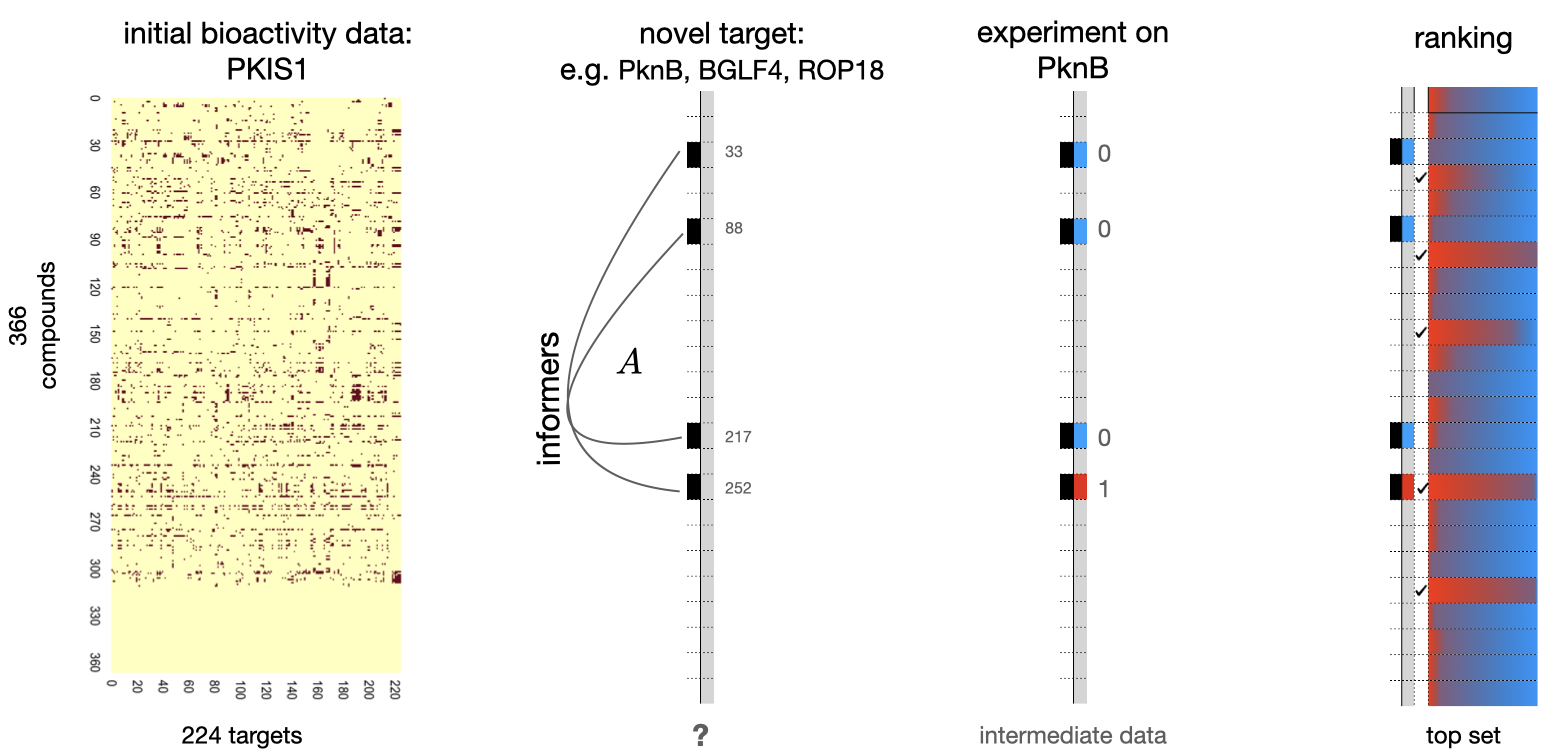
\includegraphics[width=5.5in]{Figs/IBR_scheme_PKIS1.png}
\caption{\label{fig:IBR_scheme} 
{\bf Informer-based-ranking problem:} A matrix of binary bioactivity data 
is available (left; red active, yellow inactive).  The problem is to first identify a subset of the $n$ compounds as informer compounds
that will be evaluated experimentally on new target, and then to prioritize
all the compounds for further testing after intermediate
data is obtained. }
\end{figure}

% The first-generation IBR approaches capture the statistical patterns in the initial bioactivity data by entailing a clustering of protein targets followed by feature selection to identify cluster-predictive compounds. 
% They differ in many respects, reflecting both the variety of options for each IBR step and the collaborative scheme used by \cite{zhang_predicting_2019}. 
% In spite of their heuristic formulation, these machine-learning IBR approaches exhibit impressive predictive performance when compared to baseline IBR techniques.   
% For example on the PKIS1 data set, predictive performance by machine-learning approaches exceeds baseline methods by $5\%$ to $10\%$ on average on all performance criteria, with highly significant p-values in pairwise comparison.

In~\cite{yu_bayes_2022}, the heuristic formulation is characterized as a statistical decision problem, from which a sophisticated and effective IBR method, the Bayes Optimal Informer SEt (BOISE), emerges.
BOISE aims to find an informer set that minimizes the average loss computed on hypothetical intermediate data, where the loss function is designed to penalize the inactive probabilities among top-ranked compounds and the hypothetical data is generated from a predictive distribution given the initial bioactivity data. 
% The computation of this average loss relies on a flexible sampling model where protein targets are clustered through a Chinese Restaurant Process (CRP) \citep{aldous_exchangeability_1985} and the interactions between pairs of targets and compounds are assumed to follow an independent Bernoulli distribution --- with success rate determined by both targets and compounds. 
% Such a method is evaluated on the same data sets as in~\cite{zhang_predicting_2019} and a 5\% to 10\% average improvement is achieved on all performance criteria compared to those heuristic IBR methods, with highly significant p-values in pairwise comparison.
Such a method achieved a significant improvement in performance criteria when compared to the heuristic methods in the first generation IBR approaches of~\cite{zhang_predicting_2019}.

Despite the superiority over predecessors, it remains a question whether existing BOISE method is applicable to realistic scenarios --- the largest data set that BOISE has been tested on is $224 \times 366$, while in reality thousands of candidate compounds is common in initial bioactivity data. 
When scaling up to larger data sets, a series of problems could emerge, such as the trade-off between predictive performance and computation cost, the efficiency of model sampling, and possible failures caused by floating-point error. 
% Besides, although original BOISE is optimal under the designated loss function, there is still room for improvements on both theoretical and practical aspects. 
% For instance, in original BOISE framework it's possible to have a compound tested inacitve in the intermediate data while still selected into ``top set", the set of compounds that are most likely to be active. 
% Such counter-intuitive results point to a need for alternative loss functions that can better reflect the requirements in real-world drug discovery.
% and corresponding optimal informer set under these loss functions.
In this paper, we present a BOISE variant, ``fast BOISE'', aimed to resolve these computational problems.
% The major improvements are achieved in three aspects: from a theoretical perspective, we propose a series of new loss functions that can improve the original BOISE performances; from a practical perspective, we develop the ``block BOISE'' variant for fast and efficient informer search in large wide data sets, i.e. where there are much more candidate compounds than targets. 
% An additional ``fast BOISE'' variant is designed for even faster informer search when desired informer set size is huge. 
% The proposed variants are then experimented both retrospectively and prospectively on bioactivity data that is closely related to real-world drug discovery, and the variants achieve satisfying performances with desired properties, e.g., significant reduction in computation time. 
% Theoretical improvements are achieved through the addition of new loss functions that can improve BOISE performance. 
% From a practical perspective, we introduce \emph{block BOISE} for fast and efficient informer search in ``wide'' data sets, and \emph{fast BOISE} for use when large informer sets are desired.
This method permits a decrease in computation time by orders of magnitude with no substantial loss in performance.

\section{Methodology for BOISE variants}
It may help to first recall the formulation of original BOISE. %, as it is shared throughout the section. 
Suppose $x_0 = (x_{i,j})$ is the $m\times n$ binary initial bioactivity data matrix, and $x_A = \{x_{i^*,j}:j\in A\}$ is the intermediate data derived between novel target $i^*$ and informer set $A$.
BOISE assumes $x_{i,j}$ and $x_{i^*,j}$ are Bernoulli trials governed by parameters $\theta_{i,j}$ and $\theta_{i^*,j}$, respectively. 
The key assumption of IBR framework is the similarity between targets, and hence a Chinese Restaurant Process (CRP) is applied on targets to enforce information sharing among targets while still retaining flexibility. 
BOISE models assume, therefore, that there is a partition $\mathcal{C} = \{ c_k \}$ of the $m$ initial targets, wherein each cluster $c_k$ contains identically distributed targets in the sense that $\theta_{i,j} = \sum_k \phi_{k,j}\mathbbm{1}(i\in c_k)$ for a reduced set of cluster/target parameters $\phi=\{ \phi_{k,j} \}$. 
The proposed modeling is thus:
\begin{align}
\label{eq:orig_model_structure}
\begin{split}
\mathcal{C} &\sim {\rm CRP}_m(m_0), \\  
    \phi_{k,j} & \sim {\rm Beta}(\alpha_0,\beta_0), \quad  k=1,\cdots, K, \; j=1,\cdots,n \\
x_{i,j} \mid  \mathcal{C}, \phi  & \sim {\mbox {\rm Bernoulli}} \left\{ \sum_k \phi_{k,j} \mathbbm{1}(i\in c_k) \right\},
 \quad i=1,\cdots,m, \; j=1,\cdots,n.
\end{split}
\end{align}
where Beta$(\alpha_0, \beta_0)$ is the base distribution and $m_0$ is the prior mass of CRP. 

With generative model in~(\ref{eq:orig_model_structure}), BOISE searches for the informer set $A$ that minimizes the posterior expected loss given initial $x_0$,
\begin{eqnarray}
  \label{eq:orig_orig_loss}
  L_0(A, T; \theta) = \sum_{j \in T} \left( 1- \theta_{i^*,j} \right),
\end{eqnarray}
where $A$ is the informer set and $T$ is the \textit{top set}, the set of compounds on which we will perform further experimentation in order to identify as many active compounds as possible against novel target $i^*$.
The size of informer and top set, $n_A$, and $n_T$, respectively, are predetermined as compounds are purchased and screened in batches in VS. 
In this work we consider, also, a modified version of this loss function,
\begin{eqnarray}
\label{eq:orig_loss}
L_1(A, T; \theta) = \sum_{j \in T} \left( 1- x_{i^*,j} \right).
\end{eqnarray}
The original loss function used in BOISE, $L_0$, permits odd circumstances where ``misses'', compounds observed to be inactive in the informer set, are selected for the top set. 
By replacing the $\theta_{i^*,j}$ with $x_{i^*,j}$, hits in the informer set will always be ranked first, misses will always be ranked last, and all compounds not in the informer set are ranked exactly as they were according to $L_0$.

% The design of loss function~(\ref{eq:orig_loss}) is in line with chemical screening procedure, while there may be other loss functions that coordinate better with model~(\ref{eq:orig_model_structure}).

% \subsection{BOISE with new losses}

% %\subsubsection{Loss function that coordinates $x_A$ and $T$}
% One small issue of original BOISE in practice is that inactive compounds tested in intermediate data can still be selected into top set $T$. 
% % Such confusing decision rule can be attributed to the selection of \textit{state of nature} \citep{parmigiani_decision_2009}. 
% % In loss function~(\ref{eq:orig_loss}) we select Bernoulli parameters $\{\theta_{i^*,j}\}$ as the state of nature, however, the actual bioactivities $\{x_{i^*,j}\}$ are also unknown when we make decision on informer set $A$ and $\{x_{i^*,j}\}$ is more closely related to our final goal than $\{\theta_{i^*,j}\}$. 
% One simple idea is to replace $\theta_{i^*,j}$ with $x_{i^*,j}$ in~(\ref{eq:orig_loss}). 
% We denote our new loss as $L_1(A, T; x_{i^*})$:
% \begin{eqnarray}
% \label{eq:new_loss_top_set}
% L_1(A, T; x_{i^*}) = \sum_{j \in T} \left( 1- x_{i^*,j} \right).
% \end{eqnarray}
% % then the posterior expected loss of decision rules $(A,T)$ given $x_0$ is:
% % \begin{eqnarray}
% % \label{eq:new_loss_top_set_pel}
% % {\rm PEL}(A, T) = E\left[\left. E\left\{\left. \sum_{j\in T} (1-x_{i^*,j})\,\right|\, x_0, x_A\right\}\,\right|\, x_0\right]
% % \end{eqnarray}
% % which indicates that the optimal top set rule $T^*(x_0, A, x_A)$ is to select top $n_T$ compounds with largest posterior expectation $E(x_{i^*,j}\mid x_0, x_A)$. 
% % Since $E(x_{i^*,j}\mid x_0, x_A) = x_{i^*,j}$ for $j\in A$, and for compound $j\notin A$, it can be computed through multiple conditional expectations,
% % \begin{eqnarray*}
% %     E(x_{i^*,j}\mid x_0, x_A) &=& E\left\{E(x_{i^*,j}\mid \theta, x_0, x_A)\mid x_0,x_A\right\}\\
% %     &=& E(\theta_{i^*,j} \mid x_0, x_A)
% % \end{eqnarray*}
% Recall that under $L_0(\cdot)$ loss, the best top set is the top $n_T$ compounds with largest $\hat \theta_{i^*,j} = E(\theta_{i^*,j}\mid x_0, x_A)$.
% Under $L_1(\cdot)$ the new optimal top set rule is almost the same as the old one, except for $\hat \theta_{i^*,j}$ being replaced with $x_{i^*,j}$ for $j\in A$, resolving the issue.
% % This replacement is exactly what we need as all active compounds in the intermediate data $x_A$ will be ranked at top while inactive compounds will be ranked at bottom, due to posterior expectations $\hat \theta_{i^*,j} \in (0,1)$ under Bayes model~(\ref{eq:orig_model_structure}).

% \subsubsection{Loss function compatible with ranking methods}
% Inspired by the benefit from replacing $\theta_{i^*,j}$ with $x_{i^*,j}$, 
% It may worth to reconsider the role of ``top set'' in this context.
%loss functions~(\ref{eq:orig_loss}) and~(\ref{eq:new_loss_top_set}). 
The concept of top set origins comes from chemical screening procedure, yet there is an argue around its necessity. 
The major concern is about the top set size $n_T$, as when $n_T$ changes, previous informer set will no longer be optimal % for new $n_T$-defined loss 
and another round of training and selection is needed. 
Although original BOISE is shown to be quite robust for mismatched $n_T$'s in simulation, there is no theoretical guarantee about this robustness. 
Besides, the desired output for IBR methods is a ranking of all candidate compounds, and top-set-defined losses like~(\ref{eq:orig_loss}) 
% %or~(\ref{eq:new_loss_top_set}) 
only select the top $n_T$ compounds without regard to the ordering of either the top set or the ``bottom'' set.
With such gaps between practice and decision theory, we may abandon top set $T$ in loss functions and reframe it to match the ranking procedure.

% % The lack of theoretical guarantee can also be found in the ranking procedure: for IBR methods, the desired output is a ranking of all candidate compounds, which is based on $\hat \theta_{i^*,j}$ in original BOISE. 
% % However, this ranking method is not justified by top-set-defined losses like~(\ref{eq:orig_loss}) or~(\ref{eq:new_loss_top_set}), where only top $n_T$ selected compounds are guaranteed to be ``best'', neither about their ordering nor about the other compounds. 
% % With such gaps between practice and decision theory, we may abandon top set $T$ in loss functions and reframe it to match the ranking procedure.

Due to the binary nature of bioactivity data (active/inactive), the unknown vector of interactions, $x_{i^*}$, automatically gives the true ranking of the compounds. 
The question now is how to define a loss between estimated and true ranking. 
There are a handful of ranking losses available, as summarized in~\cite{NIPS2009_chen}. 
Considering the significant number of ties in $x_{i^*}$, ranking losses based on pairwise comparison are more applicable. 
Specifically, if an estimated ranking of compounds is given from most likely to least likely to be active on the novel target, it can be represented as a $n\times n$ matrix $R$, where $n$ is the number of compounds:
\begin{eqnarray}
\label{eq:rank_matrix}
R(i,j) = \begin{cases}
  1,  &  rank(i) < rank(j) \\
  0 & rank(i) == rank(j)\\
 -1,  &  rank(i) > rank(j)
\end{cases}
\end{eqnarray}
and a new loss function for BOISE could be defined as:
\begin{eqnarray}
\label{eq:new_loss_rank}
L_2(A, R;x_{i^*}) = \sum_{j_1=1}^n\sum_{j_2=1}^n \left\{-R(j_1, j_2)(x_{i^*,j_1} - x_{i^*,j_2})\right\}_+
\end{eqnarray}
where function $\phi(z) = (z)_+$ means the positive part of $z$. Despite the complicated form as it may look like, $L_2(A,R;x_{i^*})$ has a simple interpretation: it is the number of discordant pairs between estimated ranking and true ranking. %, since the true ranking is the unknown binary vector $x_{i^*}$, and the inner part of~(\ref{eq:new_loss_rank}) is $1$ if $R$ and $x_{i^*}$ disagree on pair $(j_1, j_2)$, otherwise just $0$. 
% Notice that if $x_{i^*,j_1} = x_{i^*,j_2}$, the inner part is $0$ no matter what $R(j_1, j_2)$ is. 
Therefore, there will be many optimal rankings $R^*$ which all achieve the same minimum of $L_2(A, R;x_{i^*})$. 

% % There is a clear statistical meaning for $L_2(A,R;x_{i^*})$, as suggested in~\cite{rank_svm}: in order to measure the similarity between two rankings $r_a$ and $r_b$ of same length $m$, Kendall's $\tau$ statistic~\citep{kendall_rank_1990} is frequently used and defined as:
% % \begin{eqnarray*}
% % \tau(r_a, r_b) = \frac{P-Q}{P+Q} = 1 - \frac{2Q}{{m\choose 2}}
% % \end{eqnarray*}
% % where $P$ is the number of concordant pairs and $Q$ is the number of discordant pairs. Therefore, by penalizing the number of inversions, $L_2(A,R;x_{i^*})$ is seeking to maximize the Kendall's $\tau$ statistic between the estimated ranking $R$ and the optimal ranking $R^*$, which is closely related to $x_{i^*}$ in this case. 

% %With all the good properties of $L_2(A,R;x_{i^*})$, it is encouraging to see that optimal ranking rule is no harder than those under top-set defined losses and is consistent with the ranking method used in practice in original BOISE. 

% %%%%%%%%%%%%%%%%%%%%%%%%%%%%%%%%%%%%%%%%%%%%%%%%%%%%%%
% %%%%% APPENDIX THIS GUY %%%%%%%%%%%%%%%%%%%%%%%%%%%%%%
% %%%%%%%%%%%%%%%%%%%%%%%%%%%%%%%%%%%%%%%%%%%%%%%%%%%%%%
% % To get the optimal ranking rule $\hat R^* = \hat R^*(x_0, x_A; A)$ for fixed informer set $A$, initial data $x_0$ and intermediate data $x_A$, one may focus on the posterior expected loss condition on $x_0$ and $x_A$:

% \begin{eqnarray}
% \label{eq:new_loss_rank_pel2}
% E\{L_2(A,R;x_{i^*})\mid x_0, x_A\}= \sum_{j_1=1}\sum_{j_2=1}^n E\left[\left.\{-R(j_1, j_2)(x_{i^*,j_1} - x_{i^*,j_2})\}_+ \, \right| x_0, x_A\right]
% \end{eqnarray}
% Notice that for the inner part of~(\ref{eq:new_loss_rank_pel2}), if $j_1\in A$ and $x_{i^*,j_1} = 1$, $(x_{i^*,j_1} - x_{i^*,j_2})\geq 0$ for any possible outcomes $x_{i^*,j_2}$, thus setting $\hat R^*(j_1, j_2) = 1$ will minimize the loss corresponding to $j_1$. Similarly, if $j_1\in A$ and $x_{i^*, j_1} = 0$, setting $\hat R^*(j_1, j_2) = -1$ will be the optimal choice. Corresponding relative rankings of $j_2\in A$ can be imputed from symmetry of ranking matrix $\hat R^*$. 
% When both $j_1$ and $j_2$ are not in the informer set, the inner expectation of~(\ref{eq:new_loss_rank_pel2}) could be computed by first conditioning on $\theta$, which renders:
% \begin{eqnarray*}
% &&E\left[\left.\{-R(j_1, j_2)(x_{i^*,j_1} - x_{i^*,j_2})\}_+ \, \right| \theta, x_0, x_A\right] \\
% &=& \left(1-\theta_{i^*,j_1}\right)\theta_{i^*,j_2}\cdot \frac{1 + R(j_1,j_2)}{2} + \theta_{i^*,j_1}\left(1-\theta_{i^*,j_2}\right)\cdot \frac{1-R(j_1, j_2)}{2}\\
% &=& -\theta_{i^*,j_1}\theta_{i^*, j_2} + \theta_{i^*,j_1}\frac{1-R(j_1, j_2)}{2} + \theta_{i^*,j_2}\frac{1+R(j_1, j_2)}{2}
% \end{eqnarray*}
% and
% \begin{eqnarray*}
% &&E\left[\left.\{-R(j_1, j_2)(x_{i^*,j_1} - x_{i^*,j_2})\}_+ \, \right| x_0, x_A\right] \\
% &=&\frac{1-R(j_1, j_2)}{2} E\left(\theta_{i^*,j_1}\mid x_0, x_A\right) + \frac{1+R(j_1, j_2)}{2}E\left(\theta_{i^*,j_2}\mid x_0, x_A\right) -E\left(\theta_{i^*,j_1}\theta_{i^*, j_2}\mid x_0, x_A\right)
% \end{eqnarray*}
% The optimal relative ranking between $j_1$ and $j_2$, given $x_0$ and $x_A$, is, as shown in [APPENDIX]:
% \begin{eqnarray}
% \label{eq:optimal_rank}
% \hat R^*(j_1,j_2) = \begin{cases}
%   1,  &  \text{if } E(\theta_{i^*,j_1}\mid x_0, x_A) >  E(\theta_{i^*,j_2}\mid x_0, x_A)\\
% %   0 & rank(i) == rank(j)\\
%   -1,  &  \text{otherwise}
% \end{cases}
% \end{eqnarray}
% That is, the optimal ranking rule $\hat R^*$ in~(\ref{eq:optimal_rank}) is equivalent to rank all compounds with respect to their posterior expectation $\hat\theta_{i^*,j}$, where $\hat\theta_{i^*,j}$ is replaced with $x_{i^*,j}$ for $j\in A$. Later optimal informer sets could be sequentially selected using $\hat R^*$, with the same procedure as in~\cite{yu_bayes_2022}. 

% It may worth to note that despite the double-summation in~(\ref{eq:new_loss_rank_pel2}), it is actually a weighted sum of $\hat \theta_{i^*,j}$'s that really matters. This is due to under $\hat R^*$, if we use $r_j(x_0, x_A)$ to denote the rank of $j$th compound given $x_0$ and $x_A$, where $j\notin A$ and $r_j(x_0,x_A)\in\{1,2,\cdots,n-n_A\}$, then~(\ref{eq:new_loss_rank_pel2}) can be simplified as:
% \begin{eqnarray}
% \label{eq:new_loss_rank_simplified}
% \nonumber
% E\left\{L_2(A, \hat R^*; x_{i^*})\mid x_0, x_A\right\} &=& 2\sum_{j\notin A} \{r_j(x_0, x_A)-1\}\hat \theta_{i^*,j} - \sum_{j_1\notin A}\sum_{j_2\notin A} E(\theta_{i^*,j_1}\theta_{i^*,j_2}\mid x_0, x_A)\\
% &&
% \end{eqnarray}
% and the second term in~(\ref{eq:new_loss_rank_simplified}) is irrelevant to ranking $\hat R^*$, thus can be regarded as constant when another expectation is taken condition on $x_0$, i.e.:
% \begin{eqnarray*}
% E\left\{\left. L_2(A, \hat R^*; x_{i^*})\right | x_0\right\} &=& 2\sum_{j\notin A} E\left[\left. \{r_j(x_0, x_A)-1\}\hat \theta_{i^*,j} \right | x_0\right] - \sum_{j_1\notin A}\sum_{j_2\notin A} E(\theta_{i^*,j_1}\theta_{i^*,j_2}\mid x_0)
% \end{eqnarray*}
% Therefore, the effective part of~(\ref{eq:new_loss_rank_pel2}) is in fact a weighted sum of all the $\hat \theta_{i^*,j}$'s, with weights determined by their ranks under $\hat R^*$. 

% Some alternative pairwise loss functions are available other than the discordant pairs in $L_2(A,R;x_{i^*})$, and they have a general form under our setting:
% \begin{eqnarray*}
% L^p(A,R;x_{i^*}) = \sum_{j_1=1}^n\sum_{j_2=1}^n \phi\left\{R(j_1, j_2)(x_{i^*,j_1} - x_{i^*,j_2})\right\}
% \end{eqnarray*}
% where $\phi(\cdot)$ is a general function, with $\phi(z) = e^{-z}$ in~\cite{rank_boost} and $\phi(z) = \log(1+e^{-z})$ in~\cite{rank_net}. It's easy to prove that the optimal ranking rule will be the same as~(\ref{eq:optimal_rank}) under above examples.

% \subsubsection{Comparison of loss functions}
% There are fundamental differences between loss functions defined on top set $T$ and ranking method $R$, indicating that $L_2(A,R;x_{i^*})$ will achieve a better ranking than $L_0(A,T;\theta)$ and $L_1(A,T;x_{i^*})$. To show this, we first introduce a popular ranking measure in information retrieval that is closely related to $L_2(A,R;x_{i^*})$, the Mean Average Precision (MAP)~\citep{baeza-yates_modern_1999}. MAP measures the performance of a ranking method by averaging the precision scores of estimated ranking on all active positions for binary responses. Specifically, after rearranging the compounds with respect to estimated ranking $R$, the MAP score on two-level ranking is defined as:
% \begin{eqnarray}
% \label{eq:mean-avg-precision}
% {\rm MAP}(R; x_{i^*}) = \frac{1}{n_1}\sum\limits_{j:x_{i^*,j}=1} \frac{\sum_{k\leq j} x_{i^*,k}}{j}
% \end{eqnarray}
% where $n_1$ is the number of active responses in $x_{i^*}$. 
% In~\cite{NIPS2009_chen}, it is shown that pairwise ranking losses like~(\ref{eq:new_loss_rank}) will give a lower bound of MAP:
% \begin{eqnarray*}
% {\rm MAP}(R; x_i^*) \geq 1 - \frac{1}{n_1} L_2(A,R;x_{i^*})
% \end{eqnarray*}
% Therefore, the minimization of $L_2(A,R;x_{i^*})$ is equivalent to maximization of lower bound of MAP$(R; x_{i^*})$. 

% For top-set-defined loss functions like $L_0(A,T;\theta)$ and $L_1(A,T;x_{i^*})$, the optimal solution will lead to the maximization of $\sum_{j\in T} x_{i^*,j}$ for a fixed top set size $n_T$, and that is the same as the precision score at $n_T$. Therefore, $L_0(A, T;\theta)$ and $L_1(A,T;x_{i^*})$ only care about the precision score at a fixed level $n_T$, while $L_2(A,R;x_{i^*})$ is aiming at precision scores of all active responses, suggesting that $L_2(A,R;x_{i^*})$ should achieve better overall ranking.
% %and be more robust to other evaluation metrics like normalized enrichment factors (NEF) at different levels. 
% Following toy example will partly illustrates these differences, although we will compare these loss functions further in case studies.

% As a simple example, we compare BOISE under different loss functions using simulated bioactivity data. 
% The synthetic data is generated with the same procedure as in~\cite{yu_bayes_2022}: there are three generative scenarios with $m=30$ targets (rows) and $n=60$ compounds (columns). 
% Those scenarios differ in the construction of probability matrices $\Theta = ( \theta_{i,j} )$, with {\em fully clustered} meaning all columns share the same row clustering, {\em unclustered} meaning independent and identically distributed entries of $\Theta$, and the {\em half-clustered} case taking $30$ columns of each of these two extremes. All probabilities $\theta_{i,j}$ are sampled from prior distribution Beta$(0.1,0.9).$
% In each case we repeatedly (10 times) construct $\Theta$, and then realize the multi-Bernoulli sampling model $x_{i,j} \sim {\rm Bernoulli}(\theta_{i,j})$, conditionally independently across the matrix. To each synthetic data set we apply BOISE via leave-one-out cross-validation. The informer size $n_A$ is $3$, and $n_T = 6$ for top-set-defined losses, corresponding to $10\%$ of the total number of compounds. 
% Figure~\ref{fig:simulation_result} shows that the ordering of predictive performance is $L_2(\cdot) > L_1(\cdot) > L_0(\cdot)$ for {\em fully clustered} and {\em half-clustered} scenarios, while $L_2(\cdot)$ seems to be more sensitive to violations of target-clustering model, as it performed worst when model~(\ref{eq:orig_model_structure}) is greatly violated like in {\em unclustered} case. The same figure shows the impact of violations of the target-clustering model.    Performance degrades as a greater number of columns (compounds) violate the common target cluster assumption, but this degradation is somewhat gradual.  

% \begin{figure}[!ht]
% \centering
% 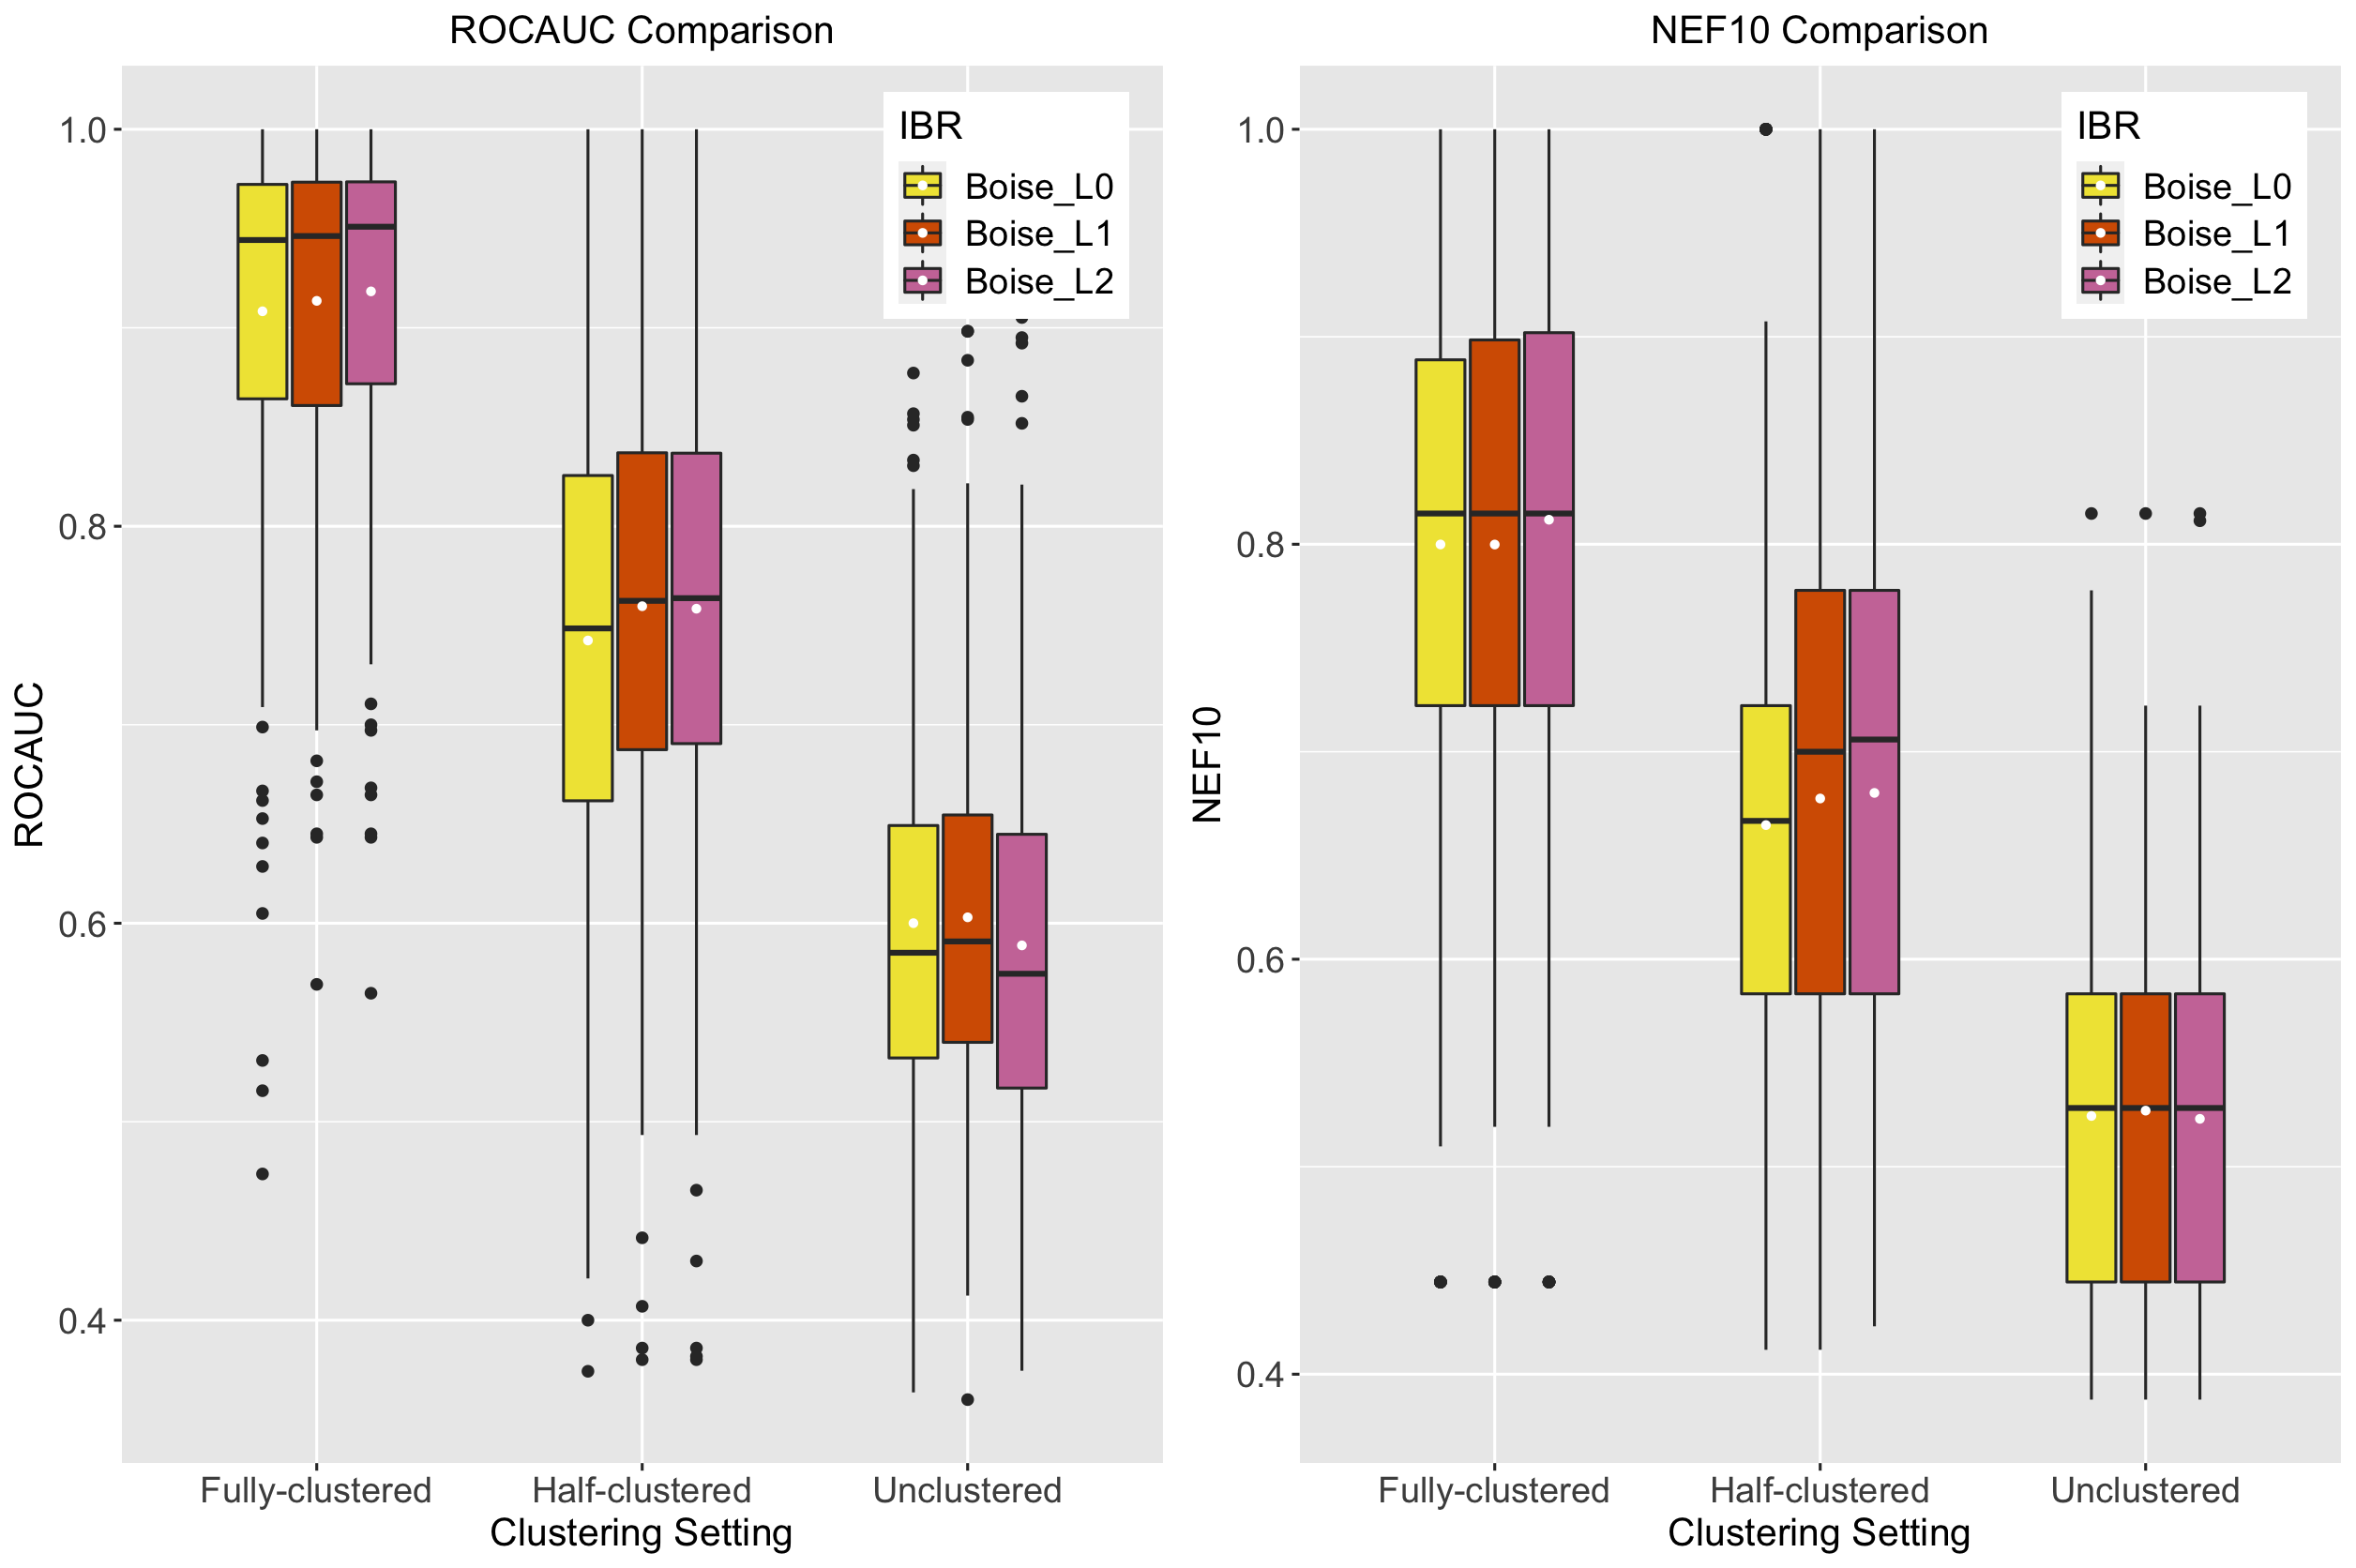
\includegraphics[width=5.0in]{Figs/new_loss_simulation_comparison.png}
% \caption{\label{fig:simulation_result} 
% {\bf Comparison of predictive performance under different losses}. 
%  We repeatedly (10 times) simulate $30 \times 60$ bioactivity data sets in three scenarios (columns: fully-clustered, half-clustered, and unclustered) which differ by the number of columns that have no cluster structure in their  $\theta_{i,j}$ settings.
%  For each synthetic data set and three loss functions, we run a BOISE cross-validation across all $m=30$ targets, and we record predictive performance with ROCAUC and NEF10.  The informer set size $n_A=3$ in all cases. } 
% \end{figure}



% \subsubsection{Alternative loss functions}
%Throughout the development of IBR methods, there are two major ideas behind the informer set selection: 
%one is to select informers sequentially, such as Regression Selection, Adaptive Selection and BOISE; the other is to select all informers from a single screening, like all baseline methods in~\cite{zhang_predicting_2019}. 
% Most recent IBR methods utilize sequential selection of informer compounds to take correlation among informers into consideration. 
% However, the informers selected from a single screening are usually easy to interpret, with a clear biochemistry meaning behind. 
% One of the most widely-used example is the frequent-hitters rule, which selects top $n_A$ most frequent hitters as the informer set and ranks all other compounds based on their similarity to those frequent-hitters. 
% %We now present a special class of loss functions that can connect frequent-hitters rule with original BOISE and reveal why it is not a good idea to use frequent hitters.
% % To get rid of sequential selection of informers, a new loss function is defined on all candidate compounds:
% It can be shown that frequent-hitters rule is the Bayes rule under new loss~(\ref{eq:frequent-hitters-loss}) with the same model~(\ref{eq:orig_model_structure}) and Haldane's improper prior $p(\phi)\propto \phi^{-1}(1-\phi)^{-1}$.
% \begin{eqnarray}
% \label{eq:frequent-hitters-loss}
% L_f(A) = \sum_{j=1}^n f_A(j),
% \end{eqnarray}
% where $f_A(\cdot)$ distinguishes informers from non-informers by:
% \begin{eqnarray*}
% f_A(j)= \begin{cases}
%   0,  &  \text{if } j\in A\\
%   \theta_{i^*,j},  &  \text{otherwise}
% \end{cases}
% \end{eqnarray*}
% % The proof is straightforward, as the posterior expected loss of~(\ref{eq:frequent-hitters-loss}) is:
% % \begin{eqnarray*}
% % {\rm PEL}(A) &=& E\left[\left. E\left\{\left. \sum_{j=1}^n f_A(j)\right| x_0,x_A\right\}\right| x_0\right]\\
% % &=& \sum_{j\notin A} E(\theta_{i^*,j} \mid x_0)
% % \end{eqnarray*}
% % with Haldane's improper prior Beta$(0,0)$, the computation will be infeasible if $i^*$ starts a new cluster. For simplicity, let's force $m_0=0$, so that novel target $i^*$ can only associate with existing clusters. If we use $m_k$ to denote the number of targets in $k$th cluster given the clustering assignment $\mathcal C$, and $a_{k,j} = \alpha_0 + \sum_{i \in c_k}x_{i,j}$ and $b_{k,j} = \beta_0 + \sum_{i\in c_k}(1-x_{i,j})$ counts actives and inactives, respectively. They are connected as $m_k = a_{k,j} + b_{k,j}$, since $\alpha_0 = \beta_0 = 0$. In that case, the posterior expectation is:
% % \begin{eqnarray*}
% % E(\theta_{i^*,j}\mid x_0) &=& E\{E(\theta_{i^*,j} \mid x_0, \mathcal C) \mid x_0\}\\
% % &=& E\left[\left.E\left\{\left.\sum_{k=1}^K P(i^*\in c_k\mid x_0, \mathcal C) E(\theta_{i^*,j} \mid x_0, \mathcal C, i^*\in c_k) \right| \mathcal C, x_0\right\} \right| x_0\right]\\
% % &=& E\left[\left.E\left\{\left.\sum_{k=1}^K \frac{m_k}{m} \cdot \frac{a_{k,j}}{a_{k,j}+b_{k,j}} \right| \mathcal C, x_0\right\} \right| x_0\right]\\
% % &=& E\left[\left.E\left\{\left.\sum_{k=1}^K \frac{a_{k,j}}{m} \right| \mathcal C, x_0\right\} \right| x_0\right]
% % = \frac{1}{m}\sum_{i=1}^m x_{i, j}
% % \end{eqnarray*}
% % From what we derived, the optimal informer set rule is to select compounds with largest posterior expectation $E(\theta_{i^*,j}\mid x_0)$, which is exactly the most frequent hitters in this setting. Therefore, frequent-hitters rule is the Bayes rule under designated priors and loss function $L_f(A)$. 

% Despite being the Bayes rule, frequent hitters are inappropriate informers as~(\ref{eq:frequent-hitters-loss}) penalizes compounds with large $\theta_{i^*,j}$'s, and that runs counter to the goal of finding compounds that are most likely to be active. This in part explains the unsatisfying performance of frequent-hitters rule as an IBR method. 
% However, $L_f(A)$ provides a family of loss functions that endorses informer selection through a single screening, if only we modify the definition of $f_A(\theta_{i^*,j})$ as:
% \begin{eqnarray*}
% \tilde f_A(j)= \begin{cases}
%   0,  &  \text{if } j\in A\\
%   g(j),  &  \text{otherwise}
% \end{cases}
% \end{eqnarray*}
% $g(\cdot)$ can be any user-specified function. The advantage of such informer selection is the fast computation, especially for large informer sizes where sequential selection can take much more time. 

% \subsection{BOISE applicable to large-scale screening}

\subsection{Block BOISE}
When scaling up BOISE to a real-world screening, the major concern is on the dramatic increase in candidate compounds: typically there is a large number of compounds tested against a relatively small number of targets, resulting in a ``wide'' bioactivity matrix $x_0$. 
%%% Just pick a smaller $m_0$? This doesn't seem right to me
% Since all compounds $j$ are assumed to share the same target clustering structure in model~(\ref{eq:orig_model_structure}), an ultra ``wide'' $x_0$ may end up with all clusters of size $1$ with high probability in a worst-case scenario. 
% Such scattered clustering will impede the information sharing among targets, which is the key factor behind superiority of original BOISE. 
In practice, the sampling of clustering structures $\mathcal C$ can be a challenge for huge number of compounds.
Therefore, the constraint that all compounds share the same target clustering may be eschewed in the presence of a ``wide'' bioactivity matrix $x_0$, and replaced with a compound-level \emph{grouping}, where each group has an individual target-level \emph{clustering} structure shared among its members.
% one feasible solution is to allow grouping among compounds, with each group of compounds having an individual target clustering structure. 
Suppose $\mathcal G = \{g_k\}$ is a partition of $n$ compounds (columns) into $K$ groups, where for each group of compounds $\{j\in g_k\}$, another partition $\mathcal C_k = \{c_{k,r}\}$ is applied on $m$ targets into $R_k$ clusters. 
For simplicity of notations, we use $x_k$ to denote the $k$th sub-matrix defined by $g_k$, where $x_0$ is the whole bioactivity data matrix. 
A generalization of model~(\ref{eq:orig_model_structure}) can be made as:

\begin{align}
\label{eq:block_boise_model}
\begin{split}
\mathcal{G} &= \{g_k\}\\  
\mathcal{C}_k & \sim {\rm CRP}_m(m_0), \quad k=1,\cdots,K\\
\phi_{r,j} \mid j\in g_k & \sim {\rm Beta}(\alpha_k,\beta_k), \quad  k=1,\cdots, K, \; r=1,\cdots, R_k \\
x_{i,j} \mid  j\in g_k, \mathcal{C}_k, \phi  & \sim {\mbox {\rm Bernoulli}} \left\{ \sum_r\phi_{r, j}\mathbbm{1}(i\in c_{k,r}) \right\},
 \quad i=1,\cdots,m, \; j=1,\cdots,n.
\end{split}
\end{align}
We use the same $m_0$ in the model but it can be different prior masses for different sub-matrices. It is easy to see that model~(\ref{eq:block_boise_model}) and~(\ref{eq:orig_model_structure}) are equivalent when $\mathcal G = \{\{1,2,\cdots,n\}\}$ is trivial. Since the bioactivity matrix generated from~(\ref{eq:block_boise_model}) is divided into blocks, the BOISE variant based on it is named as ``block BOISE''.

% %%%%%%%%%%%%%%%%%%%%%%%%%%%%%%%%%%%%%%%%%%%%%%%%%%%%%%%%%%%%%%%%%%%%%%%%%%%%%%%%%%%%%%%%%%%%
% %%%%%%%%%%%%%%%% Perhaps some image here showing group vs block vs cluster? %%%%%%%%%%%%%%%%
% %%%%%%%%%%%%%%%%%%%%%%%%%%%%%%%%%%%%%%%%%%%%%%%%%%%%%%%%%%%%%%%%%%%%%%%%%%%%%%%%%%%%%%%%%%%%

% Compound clustering is a hot topic in drug discovery, so there are many ways to form a partition of the compounds, including random clustering, such as by applying another CRP on columns.
%There are lots of ways to partition the compounds, as compound clustering is a hot topic in drug discovery. 
% In this paper, we apply the hierarchical clustering \citep{hclustering_ward_1963} on chemical structures, considering the computation cost and available compound information, and hence $\mathcal G$ is a fixed partition throughout the paper. Other compound clustering methods may be utilized and $\mathcal G$ may also be random variable, e.g. applying another CRP on columns. 
% In any case, a new algorithm compatible with given $\mathcal G$ is needed to select informers under model~(\ref{eq:block_boise_model}). 
% For that purpose, Algorithm~\ref{Alg:block_Boise_pel} below gives a general algorithm to calculate the posterior expected loss given $x_0$ (PEL$_1(x_0,A)$). 
% Notice that PEL$_2(x_0, A, x_A)$ represents the posterior expected loss given $x_0$ and $x_A$, in accordance with~\cite{yu_bayes_2022}.
% The informer scoring Algorithm~\ref{Alg:block_Boise_pel} can be conveniently altered to a compound ranking algorithm when real intermediate data $x_A$ is available. The only difference is that there is no need to sample possible outcomes $\mathbb X_{A_k}$, instead real $x_{A_k}$ is used to compute $\hat \theta_{i^*,j}$'s.

% \begin{algorithm}
% \caption{PEL Computation with compound clustering}\label{Alg:block_Boise_pel}
% \hspace*{\algorithmicindent} \textbf{Input:} Initial data $x_0$, informer set $A$, compound clustering $\mathcal G = \{g_k\}$, target clustering samples $\mathbb C_k$ from $p(\mathcal{C}_k\,|\,x_k)$.\\
% \hspace*{\algorithmicindent} \textbf{Output:} ${\rm PEL}_1(x_0,A)$ as score of informer set $A$. 
% \begin{algorithmic}[1]
% \State Define an empty list \textbf{Scores} to store possible intermediate data $x_A$'s, together with their occurrence probability $P(x_A\mid x_0)$ and posterior expectations $\hat \theta_{i^*,j}=E( \theta_{i^*,j} | x_A, x_0)$.
% \For{each $g_k$ in $\mathcal G$}
%         \State Determine $A_k = A\bigcap g_k$ . \Comment{Sub-informer set}
%         \If{$A_k == \emptyset$ }
%             \State Set $x_{A_k} = {\rm NULL}$ and $P(x_{A_k}|x_k) = 1$;
%             \State Compute $\hat \theta_{i^*,j}=E( \theta_{i^*,j} \mid x_k)$ by averaging $E(\theta_{i^*,j}\mid x_k, \mathcal C_k)$ for $\mathcal C_k \in \mathbb C_k$.
%         \Else
%             \State Sample possible outcomes of $\mathbb X_{A_k}$ from $p(x_{A_k}\mid \mathcal C_k, x_k)$;
%             \For{each distinct $x_{A_k}$ in $\mathbb X_{A_k}$}
%                 \State Compute $P(x_{A_k} \mid x_k)$ and $\hat \theta_{i^*,j}$ in the same way as in original BOISE;
%             \EndFor
%         \EndIf
%         \State Update \textbf{Scores} by appending all distinct $x_{A_k}$ to previous partial outcomes of $x_A$. 
%         \State Update corresponding occurrence probabilities and fill in $\hat \theta_{i^*,j}$'s for new compounds.
% \EndFor
%     \State Calculate PEL$_1(x_0,A)$ by weighted averaging PEL$_2(x_0,A,x_A)$ over all possible $x_A$ in \textbf{Scores}. The weights are occurrence probabilities.
% \end{algorithmic}
% \end{algorithm}

% In Algorithm~\ref{Alg:block_Boise_pel}, although compounds are separated into  groups, the computation of occurrence probability $P(x_A\mid x_0)$ and posterior expectation $\hat \theta_{i^*,j}$ is straightforward as generating models on each sub-matrix $x_k$ are independent.
% The complexity is on ranking of $\hat \theta_{i^*,j}$'s, as we need to store the intermediate results and merge all pieces together to achieve a final ranking of the whole set of compounds. 
% The space complexity could be potential bottleneck due to $2^{n_A}$ possible $x_A$ samples after merging, each comes with a length-$n$ vector of $\hat \theta_{i^*,j}$'s. If memory requirement becomes unacceptable for large $n_A$, one could set an upper bound on the number of distinct $x_A$'s and only store the most probable samples when merging different sub-matrices. This additional step will keep memory and time complexity both under control with least loss in accuracy. 

% Complicated as it may seem, block BOISE is computationally more efficient than original BOISE. The advantage comes from breaking $x_0$ and $A$ into pieces and sampling from each sub-matrix. Original BOISE samples possible $x_A$'s in whole and hence is faced with a vast sampling space of order $\mathcal O(2^{n_A})$; in contrast, $A$ is broken into $A_k$'s for block BOISE and the sampling space is $\mathcal O(2^{n_1} + \cdots + 2^{n_K})$, where $n_1+n_2+\cdots +n_K = n_A$. The reduction in sampling space is significant for large $n_A$'s. For example, when $n_A=15$, the size of sampling space for original BOISE is $2^{15} = 32768$; however, if informer set is equally broken into $3$ pieces, the size of sampling space is reduced to $3\times 2^5 = 96$. This reduction in sampling space will lead to more efficient computation for block BOISE, as is confirmed in case studies. The computation efficiency comes with a price, that is we assume independence among sub-matrices. The assumption is only reasonable if connections among groups of compounds are weak, and hence a reliable chemical clustering is important.
\subsection{Fast BOISE}
% Although block BOISE is able to handle large number of compounds, it still selects informers through a sequential selection. 
An exhaustive search for the optimal size $n_A$ informer set is intractable.
BOISE, therefore, utilizes sequential selection by selecting, first, the optimal size 1 informer set, then iteratively adding the next best compound given the current informer set until the desired quantity is reached.
This sequential selection becomes problematic as the size of the informer set increases.
For $n_A \approx 100$ or $1000$, sequential selection can take a huge amount of time. 
Even if the chemical screening researchers are willing to wait for the selection, it is better to have a fast version that provides a rough estimation of the performance when $n_A$ increases, and that can serve as a reference for the design of experiments. 
To meet this end, we introduce a class of loss functions that are capable of non-sequential selection:
% \begin{eqnarray}
% \label{eq:frequent-hitters-loss}
% L_f(A) = \sum_{j=1}^n f_A(j),
% \end{eqnarray}
% where $f_A(\cdot)$ distinguishes informers from non-informers by:
% \begin{eqnarray*}
% f_A(j)= \begin{cases}
%   0,  &  \text{if } j\in A\\
%   % \theta_{i^*,j},  &  \text{otherwise}
%   g(j), &\text{otherwise}
% \end{cases}.
% \end{eqnarray*}

\begin{eqnarray}
  \label{eq:fast-boise-loss}
  L_f(A) = \sum_{j\not\in A}f(j)
\end{eqnarray}

% In that direction, loss functions of the form~(\ref{eq:frequent-hitters-loss}) can be utilized to avoid the sequential selection and save time. A carefully designed function $g(j)$ should replace the $\theta_{i^*,j}$ term in $f_A(j)$, so that the performance of the ``fast BOISE" can be related to original or block BOISE in some ways. 
In the discussion of~\cite{yu_bayes_2022}, an inspection into the posterior expected loss computation shows that the posterior probability $p_k = P(i^*\in c_k\,|\,\mathcal{C},x_0,x_A)$ may effectively score the informer sets,
since $(p_0,p_1,\cdots,p_K)$ constitute the conditional distribution of the cluster label for target $i^*$ given $\mathcal C$, $x_A$ and $x_0$, and posterior expectations $E(\theta_{i^*,j}\,|\, x_0,x_A,\mathcal{C},i^*\in c_k)$ have a limited role in selecting top set $T^*(A,x_A,x_0)$. 
An approximate version of BOISE is then developed using the entropy of $p$, guided by ID3 decision tree algorithm in~\cite{quinlan_induction_1986}. 
% The performance of that approximate method is similar to the original BOISE, thus one may borrow the same idea in developing the fast BOISE method. 
Suppose random variable $L_{i^*}(\mathcal C)$ denotes the cluster label for target $i^*$ given clustering structure $\mathcal C$, and $X_{i^*, j}$ denotes the interaction of $j$th compound against target $i^*$.
A reasonable choice of loss is $L_{\tilde f}(A)$ where:
\begin{eqnarray}
\label{eq:fast_boise_mutual_info}
\tilde f(j) = D_{KL}\left[P\left\{L_{i^*}(\mathcal C) \,\mid\, X_{i^*,j}\right\} \middle\| P\{L_{i^*}(\mathcal C)\} \right]
\end{eqnarray}
where $D_{KL}(\cdot)$ is the Kullback–Leibler (KL) divergence \citep{KL-divergence}, $P\{L_{i^*}(\mathcal C)\}$ is the prior distribution of cluster label for target $i^*$ (that is the CRP prior) and $P\left\{L_{i^*}(\mathcal C) \,\mid\, X_{i^*,j}\right\}$ is the conditional distribution of cluster label given the outcome $X_{i^*,j}$. 
Notice that this conditional distribution is different from previous $p=(p_0,p_1,\cdots,p_K)$, which is conditioned on the whole intermediate data $x_A$. 
The KL divergence measures the information gain of $L_{i^*}(\mathcal C)$ when $X_{i^*,j}$ is known, and the posterior expected loss of $L_{\tilde f}(A)$ with regard to~(\ref{eq:fast_boise_mutual_info}) can be computed via double expectation:
\begin{eqnarray*}
{\rm PEL}_1(A) &=& E\left[\left. E\left\{\left. \sum_{j\not\in A}^n \tilde f(j)\right| x_0,x_A\right\}\right| x_0\right]\\
&=& \sum_{j\notin A} E[D_{KL}\left[P\left\{L_{i^*}(\mathcal C) \,\mid\, X_{i^*,j}\right\} \middle\| P\{L_{i^*}(\mathcal C)\} \right] \mid x_0]\\
&=& \sum_{j\notin A} E\left[E\left[D_{KL}\left(\cdot \right)\mid \mathcal C, x_0\right]\mid x_0\right]
\end{eqnarray*}
and the inner part of last equation, $E\{D_{KL}(\cdot)\mid \mathcal C, x_0\}$, is the mutual information (MI) between $L_{i^*}(\mathcal C)$ and $X_{i^*,j}$ conditional on $\mathcal C$, which is in line with selection criteria in ID3 algorithm when clustering assignment $\mathcal C$ is given.  

The Bayes rule of revised $L_{\tilde f}(A)$ would be to select top $n_A$ compounds $j$ with largest expected mutual information between cluster label $L_{i^*}(\mathcal C)$ and $X_{i^*,j}$, the potential outcome on $j$. 
Although integrated fast BOISE method is not the same as ID3 algorithm which is also a sequential selection with greedy search, the selected informers are most likely to cover the real ``key" compounds for large informer size $n_A$, and that is exactly the scenario under which fast BOISE is developed. 
In case studies, fast BOISE is shown to be closely related to original BOISE with an example target, and it achieves comparable performance considering its reduction in computation time by orders of magnitude. 

\section{Empirical studies}
\subsection{FDA data set}
The FDA data set is a newly constructed data set between FDA approved drugs and Pubchem bio-assays \citep{pubchem_bioassay_2017}. 
It contains bioactivity information on $688$ targets and $2002$ compounds, with a missing rate of $75.8\%$ and active rate of $5.2\%$. 
We select compounds from the Selleck FDA set with at least $1$ active and inactive label on the frequently tested Pubchem Bioassay targets (tested on $\geq 1000$ compounds). 
After that, targets are selected from those frequently tested assays with at least $2$ active and inactive labels on the selected compounds. 
FDA approved drugs are most common starting points in drug discovery process, and we compare variants of BOISE in both retrospective and prospective ways on this FDA data set.

% \subsubsection{Analysis of BOISE informers}
% The informer selection is like a black box in original BOISE due to the complicated posterior expected loss function, and one may hope to understand what characteristic makes a compound more likely to be an informer. As an illustration of how original BOISE selects informers, a test target, AID-540308, is randomly sampled from FDA data set, with the other $687$ targets constituting the training data. 
% After original BOISE is applied on this test target, $100$ clustering assignments are sampled from CRP. These clustering samples can be visualized by an adjacency matrix with each entry $(i,j)$ being the frequency that $i$th and $j$th target are in the same cluster. An investigation into the adjacency matrix finds $5$ groups of  targets that are always clustered together, i.e. the frequency in adjacency matrix is $1$. The sizes of these $5$ target groups are $(23,9,16,8,30)$, respectively, and Table~\ref{tab:avg_active_rates_example} below summarizes the average active rates of first $6$ informers within each group:

% \begin{table}[htbp]
% \caption{\label{tab:avg_active_rates_example}  {\bf Average active rates of first $6$ informers within $5$ groups of targets that are always clustered together for test target AID-540308.} }
% \begin{tabular}{r|rrrrrr}
% \multicolumn{1}{c}{} & 
% \multicolumn{1}{c}{CID-5288209} & 
% \multicolumn{1}{c}{CID-5281708} & 
% \multicolumn{1}{c}{CID-71188} & 
% \multicolumn{1}{c}{CID-4212} & 
% \multicolumn{1}{c}{CID-32798} & 
% \multicolumn{1}{c}{CID-2722} 
% \\
%  \hline
%  G1 & 0 & NA & NA & 1 & NA & 0\\
%  G2 & 0.83 & 0 & 0 & 1 & 0 & 0\\
%  G3 & 1 & 0.75 & 0 & 1 & 0.58 & 1\\
%  G4 & 0 & 0 & 0 & 0 & 0 & 0\\
%  G5 & 1 & 0 & 0 & 1 & 0 & 0.95\\ 
%  \hline
% \end{tabular}
% \end{table}
% The average active rates are either close to $0$ or close to $1$, with a substantial divergence among groups. Furthermore, these groups can be well distinguished from bioactivities on $4$ out of the first $6$ informers, as shown in Fig~\ref{fig:boise_illus}:
% \begin{figure}[!ht]
% \centering
% 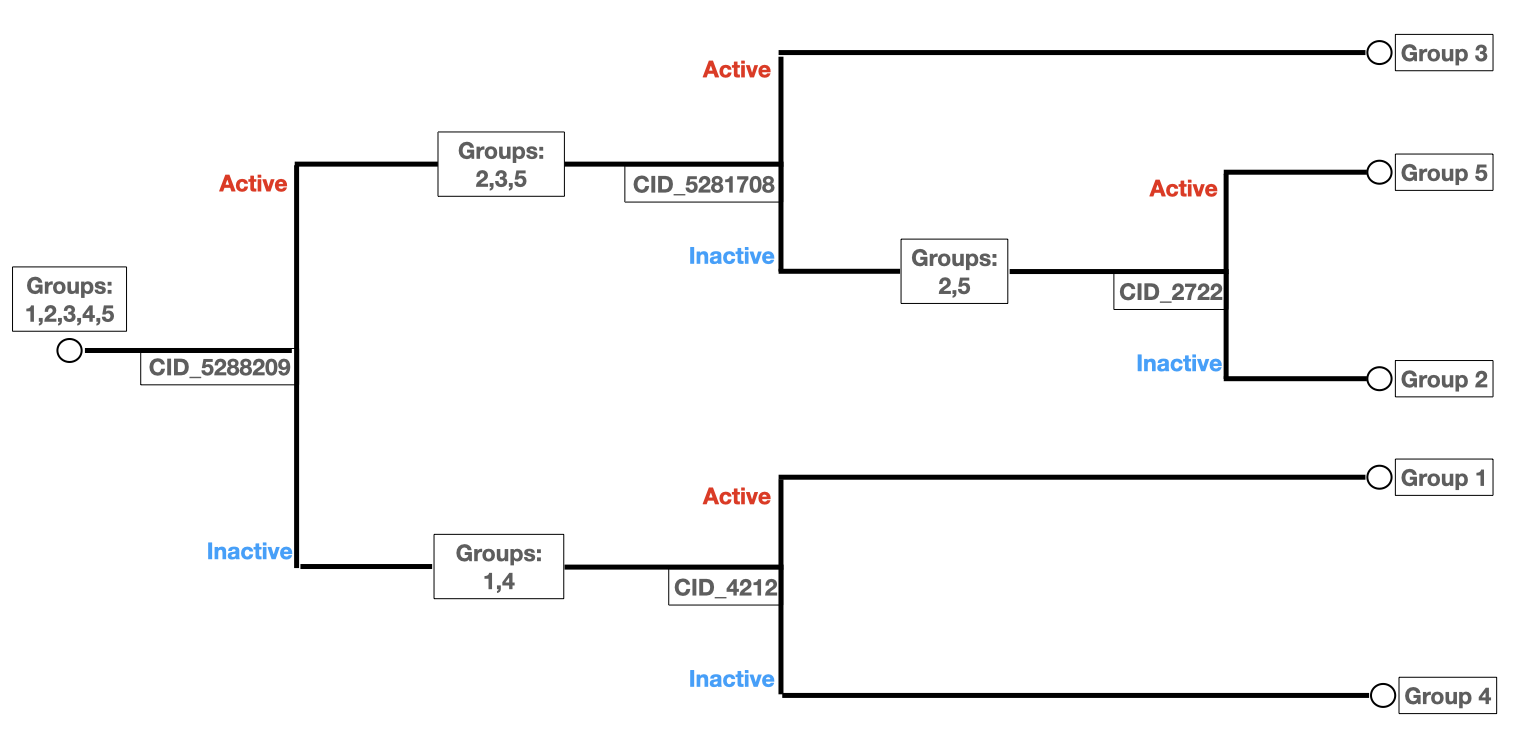
\includegraphics[width=5.0in]{Figs/decision_tree_boise_illustration.png}
% \caption{\label{fig:boise_illus} 
% {\bf Illustration of how $5$ target groups can be distinguished using responses on $4$ informers out of first $6$ for sampled test target AID-540308}}
% \end{figure}

% In other words, the informers selected by original BOISE are more likely to be compounds that can distinguish the target clusters, and that is in accordance with fast BOISE in~(\ref{eq:fast_boise_mutual_info}) where compounds with largest expected mutual information is selected, since mutual information measures the reduction in the entropy of new target's cluster label if response $X_{i^*,j}$ is known. Although interaction among informers is neglected in fast BOISE, the informers selected in both methods share similar characteristics. Given the sparse nature of original bioactivity data $x_0$, there should be limited number of ``key'' compounds, and fast BOISE is able to cover those ``key'' compounds earlier than other fast-selection methods when $n_A$ increases.

\subsubsection{Retrospective analysis}
To evaluate and compare BOISE variants retrospectively, $60$ targets are randomly selected from FDA data set and tested in a way that the selected target plays the role of $i^*$, while the other $687$ targets provide data $x_0$. 
%% Does this bit mess stuff up?
Due to the high missing rate of FDA data set, each sampled target is required to have at least $400$ complete 
responses to become a test target. 
% Well this isn't the reason, right....?
Informer selection is restricted to non-missing compounds of each test target, as incomplete $x_A$ could lead to unexpected results. 

% The first numerical experiment is to compare BOISE with $3$ loss functions: $L_0(A,T;\theta)$ in~(\ref{eq:orig_loss}), $L_1(A, T;x_{i^*})$ in~(\ref{eq:new_loss_top_set}) and $L_2(A,R;x_{i^*})$ in~(\ref{eq:new_loss_rank}). 
% Fig~\ref{fig:roc_nef10_compar_L012} plots the average performance of all $3$ BOISE variants on $60$ test targets, with informer size $n_A$ increasing from $1$ to $15$. 
% Baseline method is a simple ranking method where compounds are ranked based on their average active rates. 
% The evaluation metrics are same as in~\cite{yu_bayes_2022}, with ROCAUC evaluating the overall ranking performance and NEF10 evaluating the performance on top $10\%$ ranked compounds. 
% On the first $5$ informers, top-set-defined losses $L_0(\cdot)$ and $L_1(\cdot)$ are better than ranking loss $L_2(\cdot)$, while the latter catch up afterwards. To be more specific, when informer size becomes larger, $L_2(\cdot)$ achieves best overall ranking, and $L_1(\cdot)$ achieves best ranking on top $10\%$ compounds. The original BOISE method (that is $L_0(\cdot)$) is kind of left behind by two variants after informer size $7$. 
% \begin{figure}[!ht]
% \centering
% 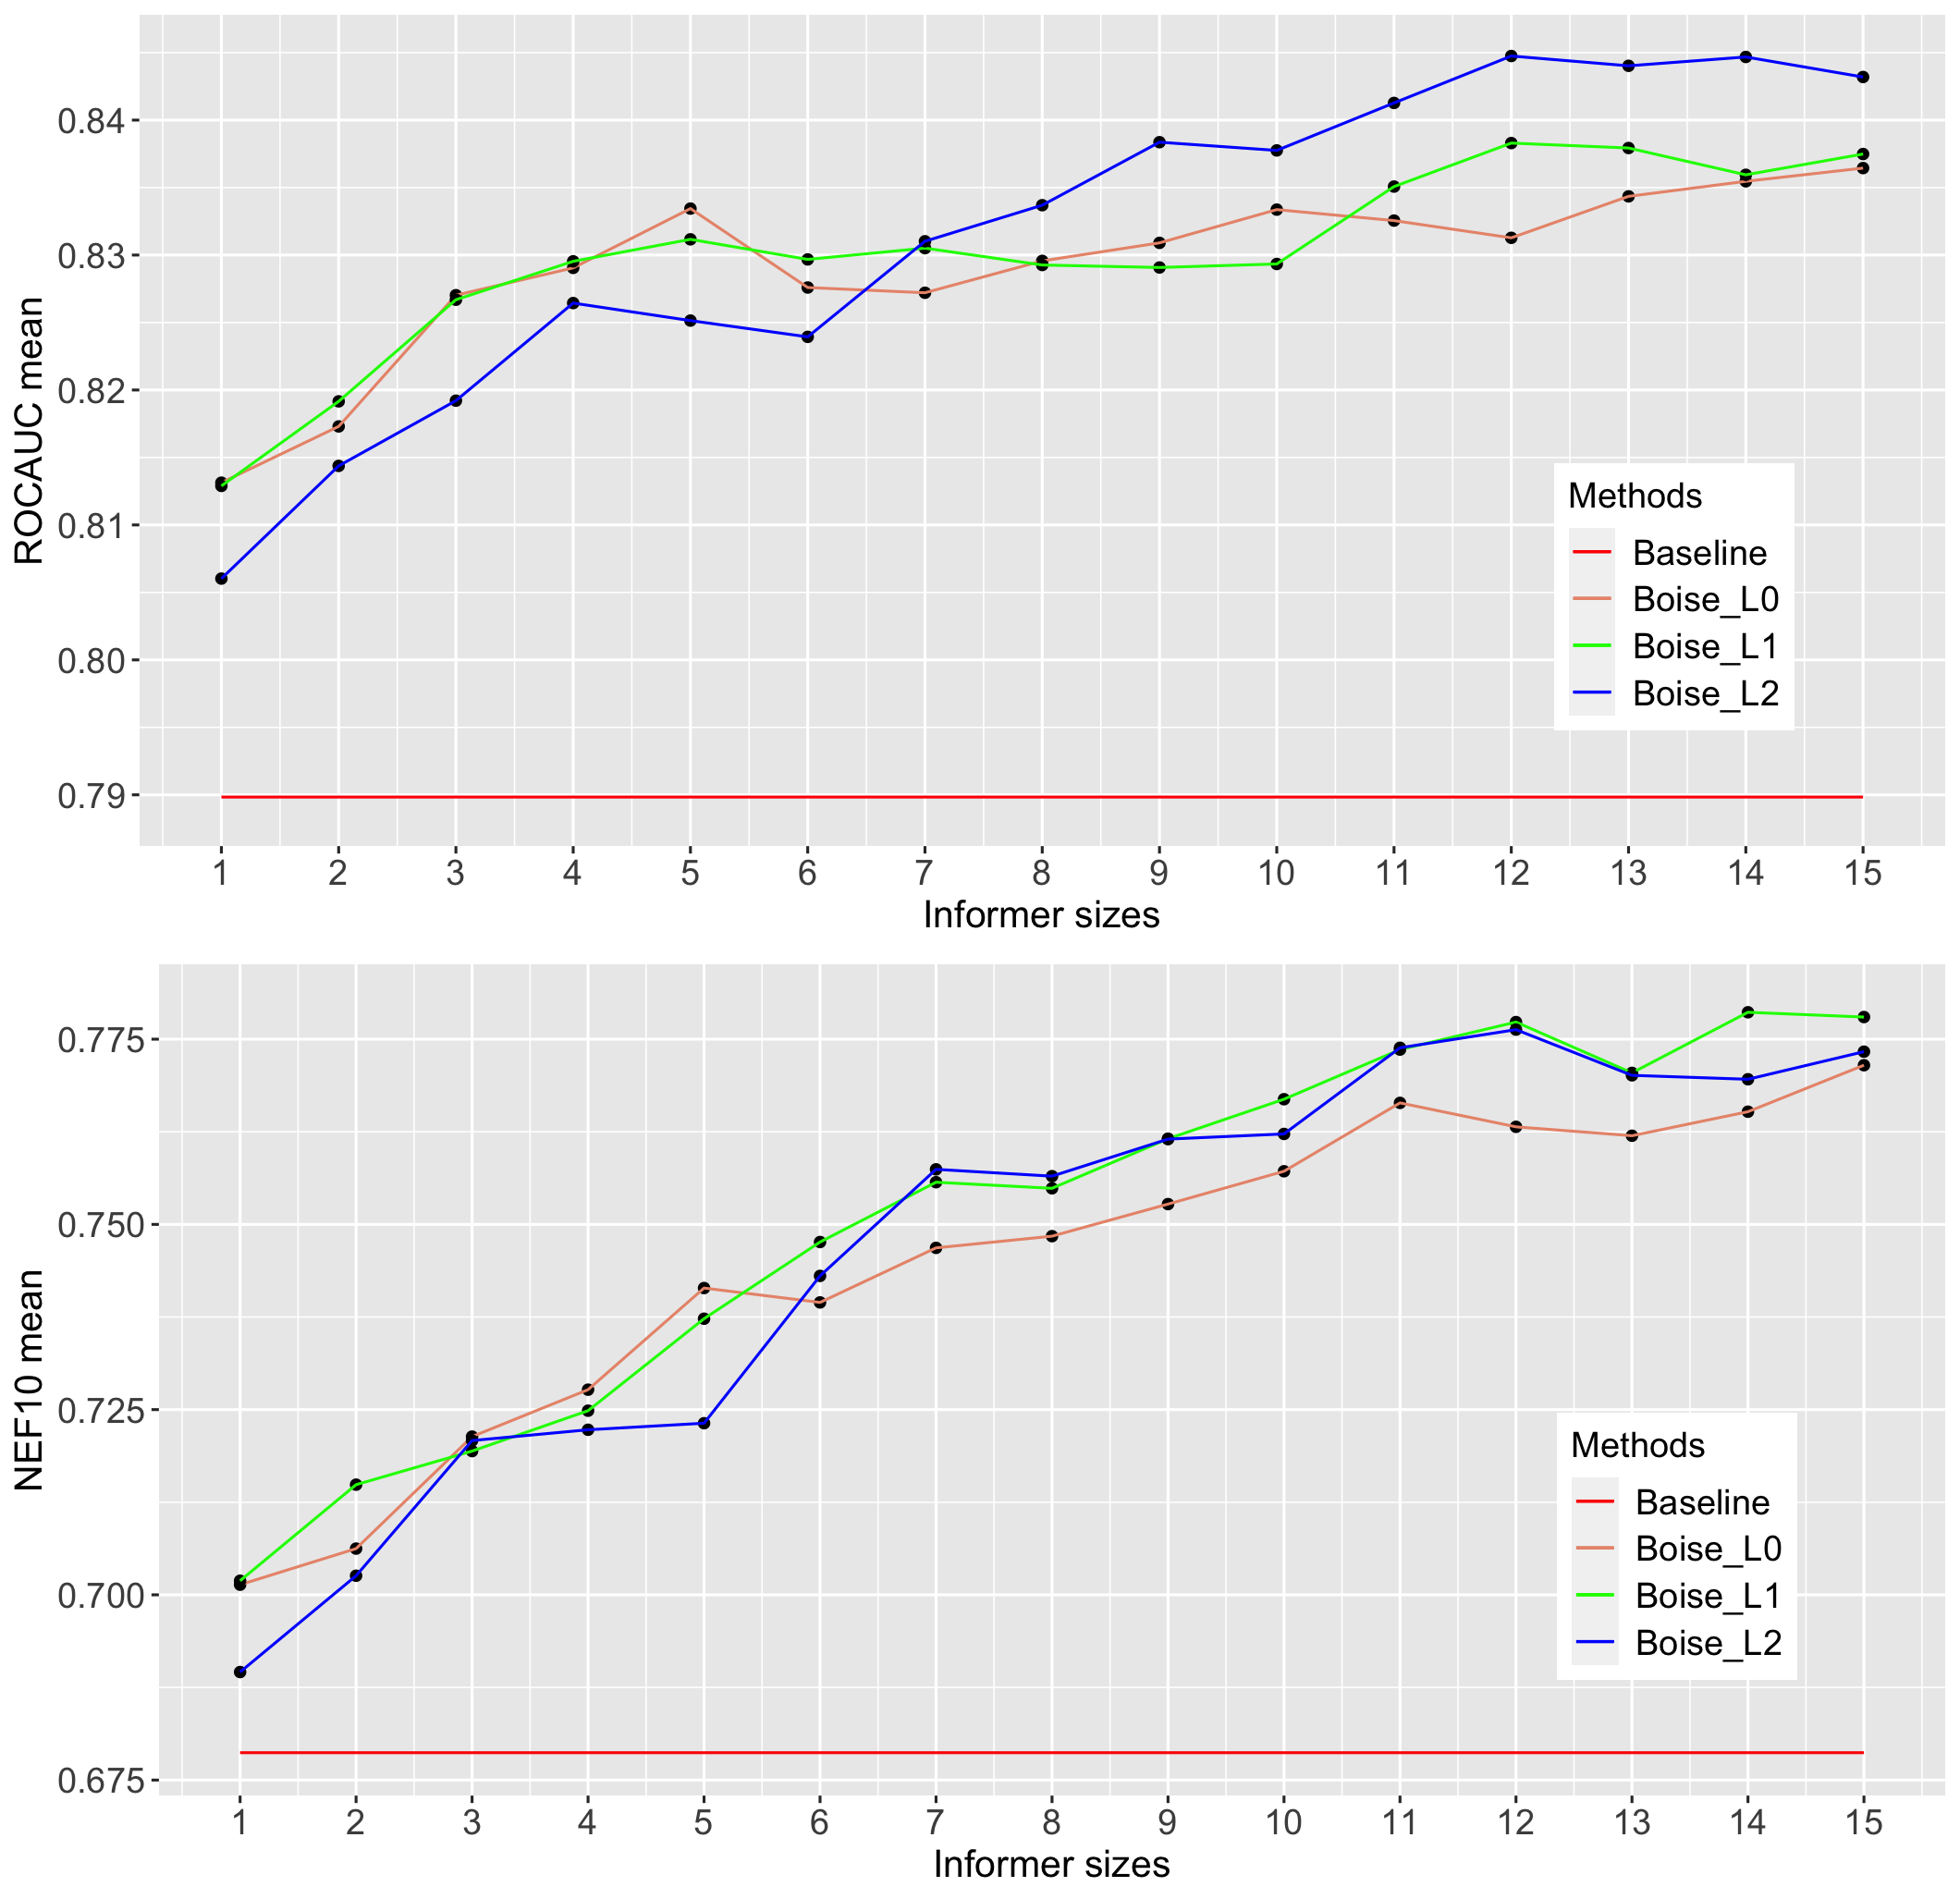
\includegraphics[width=5.0in]{Figs/roc_nef10_comparison_w_L012.png}
% \caption{\label{fig:roc_nef10_compar_L012} 
% {\bf Comparison of NEF10 and ROCAUC for BOISE with $3$ different loss functions on FDA data set when $n_A$ increases from $1$ to $15$}. }
% \end{figure}
% The leading position of $L_1(\cdot)$ on NEF10 and $L_2(\cdot)$ on ROCAUC is understandable from Section 2.1.3, as $L_2(\cdot)$ aims to maximize the mean average precision while $L_0(\cdot)$ and $L_1(\cdot)$ only care about the precision score in top $10\%$ ranked compounds. 
% Such difference can be further illustrated when performances on other levels are of interest for top-ranked compounds. For example, Fig~\ref{fig:diff_nef_compar_L012} compares the same $3$ BOISE variants on NEF10, NEF20 and NEF30, where top $10\%$, $20\%$ and $30\%$ of ranked compounds are taken into account, respectively.
% It's no wonder to see that $L_1(\cdot)$ leads on NEF10, while $L_2(\cdot)$ is the best on NEF20 and NEF30 for informer size $n_A$ large enough.
% \begin{figure}[!ht]
% \centering
% 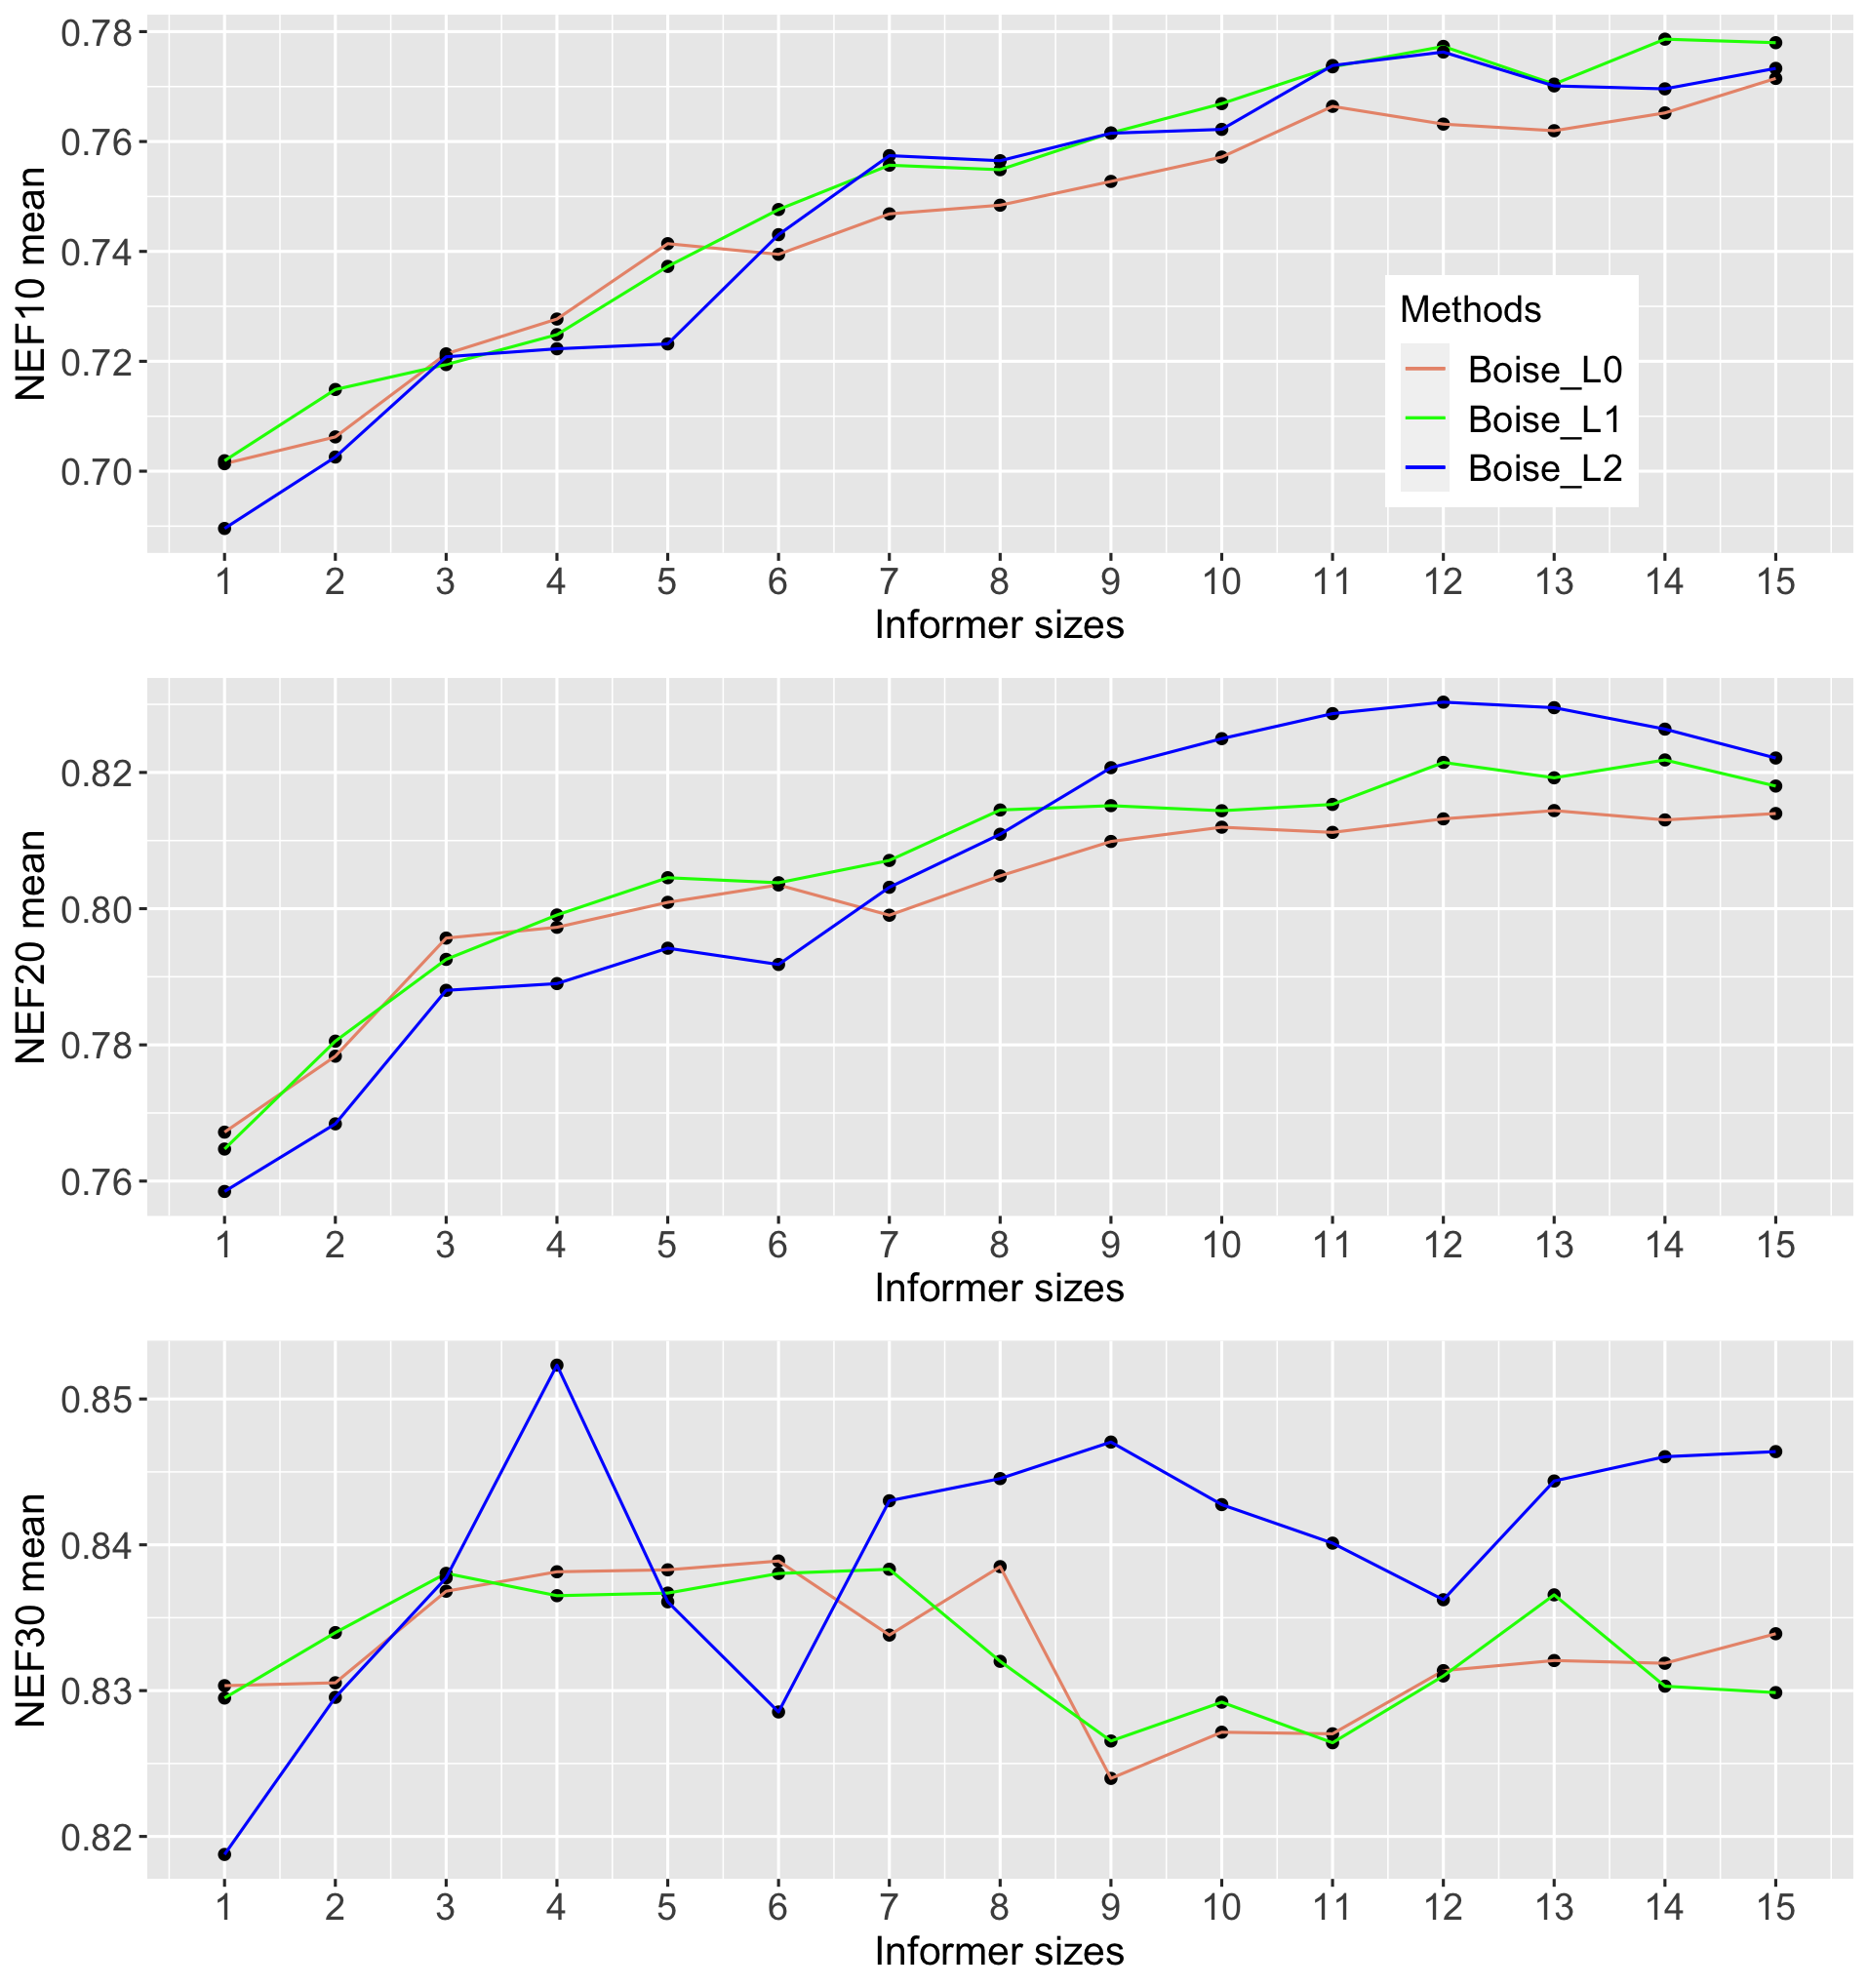
\includegraphics[width=5.0in]{Figs/diff_nef_compar_L012.png}
% \caption{\label{fig:diff_nef_compar_L012} 
% {\bf Comparison of NEF10, NEF20 and NEF30 for BOISE with $3$ different loss functions on FDA data set when $n_A$ increases from $1$ to $15$}. }
% \end{figure}

The next experiment evaluates the performance of block BOISE and fast BOISE on FDA data set. 
To get compound clustering $\mathcal G$ in block BOISE, the divisive analysis clustering (DIANA) is applied on Morgan (ECFP) fingerprints of compounds with 2048 bit length and radius$=3$~\citep{fingerprints_rogers_2010}.
DIANA is a top-down approach of hierarchical clustering where all data points are initially assigned a single cluster and then split into groups~\citep{kaufman_finding_2005}. 
The chemical fingerprint of a compound is a fixed length binary vector (2048 in this case) where each position indicates the presence/absence of certain molecule. We apply Jaccard distance on chemical fingerprints  to define similarity between two compounds in this experiment, and Silhouette score~\citep{Rousseeuw_Silhouettes_1987} is used to determine the number of clusters. After evaluating on $K=2\cdots 25$ for DIANA clustering, $K=23$ achieves highest Silhouette score, thus $2002$ FDA compounds are partitioned into $23$ groups. 

With this partition $\mathcal G$, block BOISE and fast BOISE are applied on the same $60$ test targets sampled from FDA data set. In this experiment, $L_1(A, T;x_{i^*})$ is used for block BOISE. The left panel of Fig~\ref{fig:roc_nef_compar_block_fast} shows average performances of block and fast BOISE without partition $\mathcal G$ for $n_A = 1\cdots 20$, while the right panel shows the average performances with partition $\mathcal G$ for $n_A = 1\cdots 30$. 

\begin{figure}[!ht]
\centering
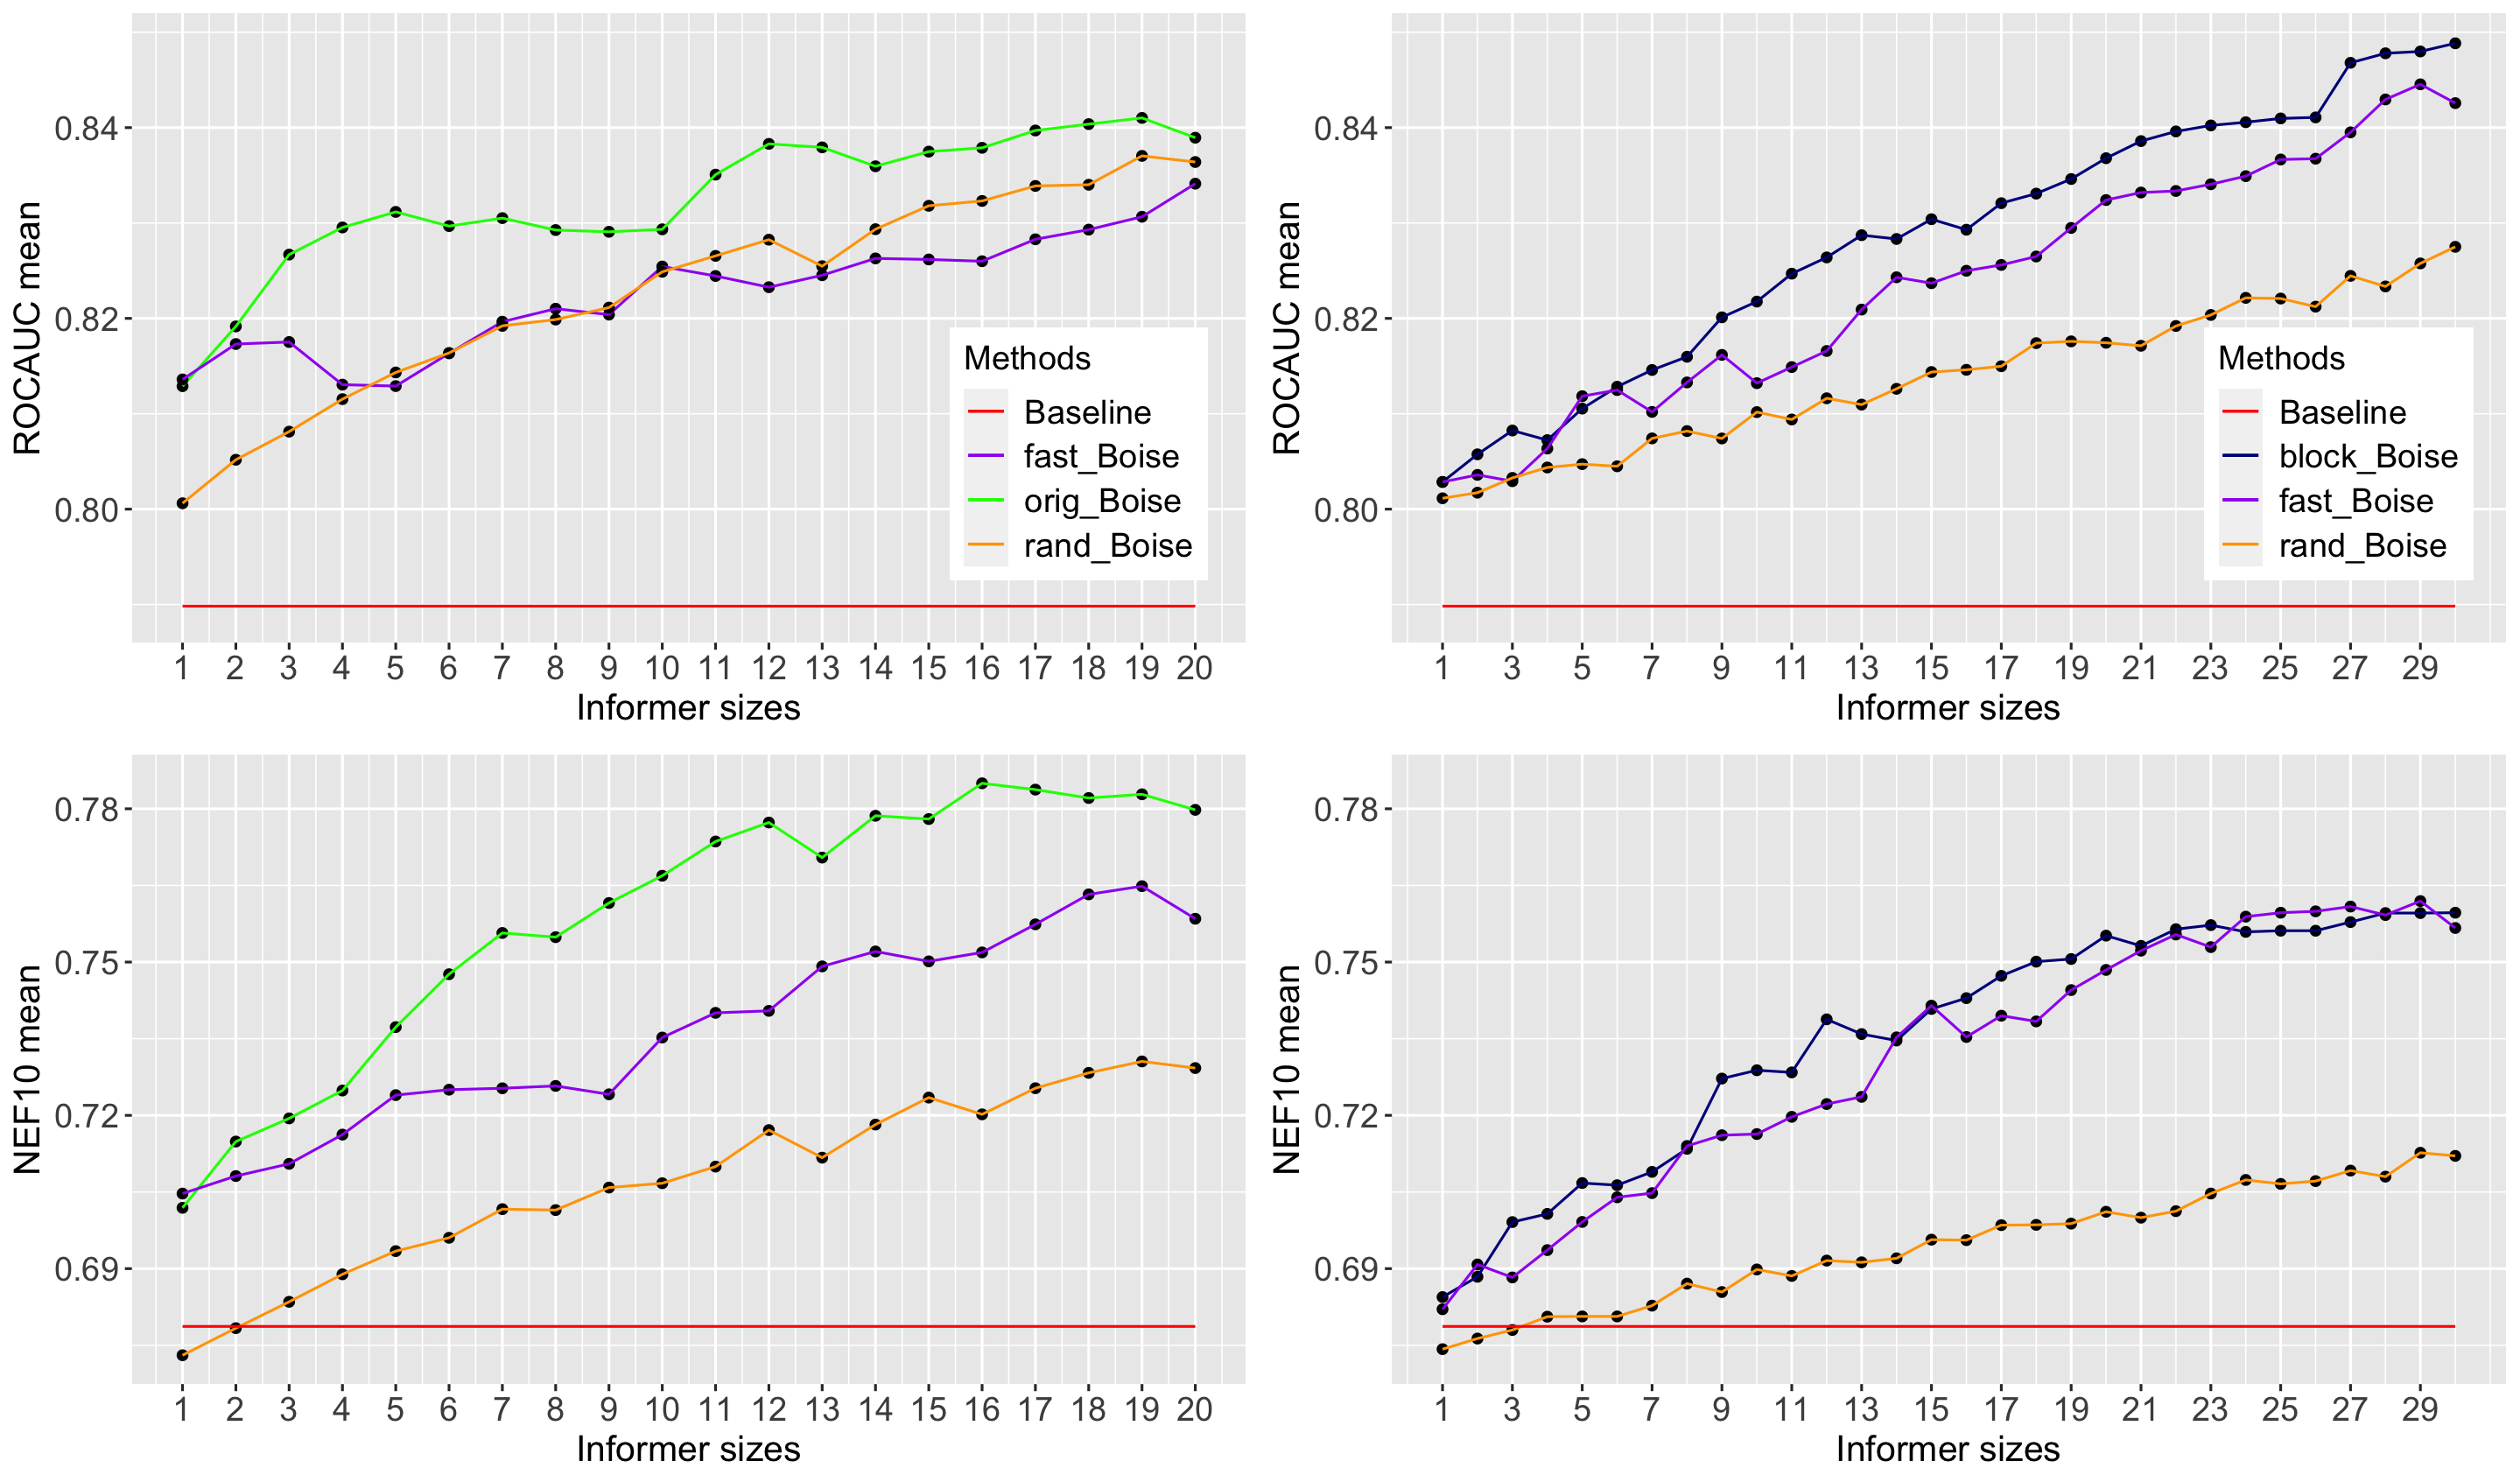
\includegraphics[width=5.0in]{Figs/roc_nef10_comparison.png}
\caption{\label{fig:roc_nef_compar_block_fast} 
{\bf Comparison of block BOISE, fast BOISE and baseline randomly selected informers when $n_A$ increases}.}
\end{figure}
In Fig~\ref{fig:roc_nef_compar_block_fast}, ``orig-BOISE" refers to the traditional BOISE with loss function $L_1(A, T;x_{i^*})$ because block BOISE and traditional BOISE are equivalent when $\mathcal G$ is trivial, and original BOISE stops at informer size $20$ due to unacceptable running time and stagnant performances. Such stagnation seems not to happen for block BOISE, even when $n_A$ increases to $30$. ``Rand-BOISE" is a baseline method where informers are randomly sampled from available compounds, and each point is the average performance of $25$ random samples for each test target.
BOISE with $L_1(A, T;x_{i^*})$ loss is still the best method under NEF10 metric, while block BOISE steadily achieves better ROCAUC after $n_A=20$. As for fast BOISE, it performs slightly better without the restriction of compound partition $\mathcal G$. Although fast BOISE is not so good as traditional BOISE or block BOISE, it is quite close to block BOISE and can significantly reduce the informer search time, as shown in Table~\ref{tab:running_time}. 

\begin{table}[htbp]
\caption{\label{tab:running_time}  {\bf Computation time of posterior expected loss evaluation in different BOISE variants for 20th informer selection.} The computation time below refers to the evaluation time on HTCondor for one candidate compound during the search of 20th informer. }
\begin{tabular}{r|rr}
\multicolumn{1}{c}{BOISE variants} & 
\multicolumn{1}{c}{Average time (min)} & 
\multicolumn{1}{c}{Max time (min)} 
\\
 \hline
 orig-BOISE &  $180$ & $240$\\
 block-BOISE & $30$ & $45$ \\
 fast-BOISE & $<1$ & $<1$\\
 \hline
\end{tabular}
\end{table}

In the upper left plot of Fig~\ref{fig:roc_nef_compar_block_fast}, the ROCAUC of randomly selected informers is sometimes better than fast BOISE without compound clustering $\mathcal G$, and this is by accident, as in Fig~\ref{fig:fast_rand_200_informer} fast BOISE shows a consistent superiority over randomly selected informers for a larger range of informer sizes.
Fig~\ref{fig:fast_rand_200_informer} also shows that fast BOISE will achieve satisfying performances when informer size becomes larger. 


\begin{figure}[!ht]
\centering
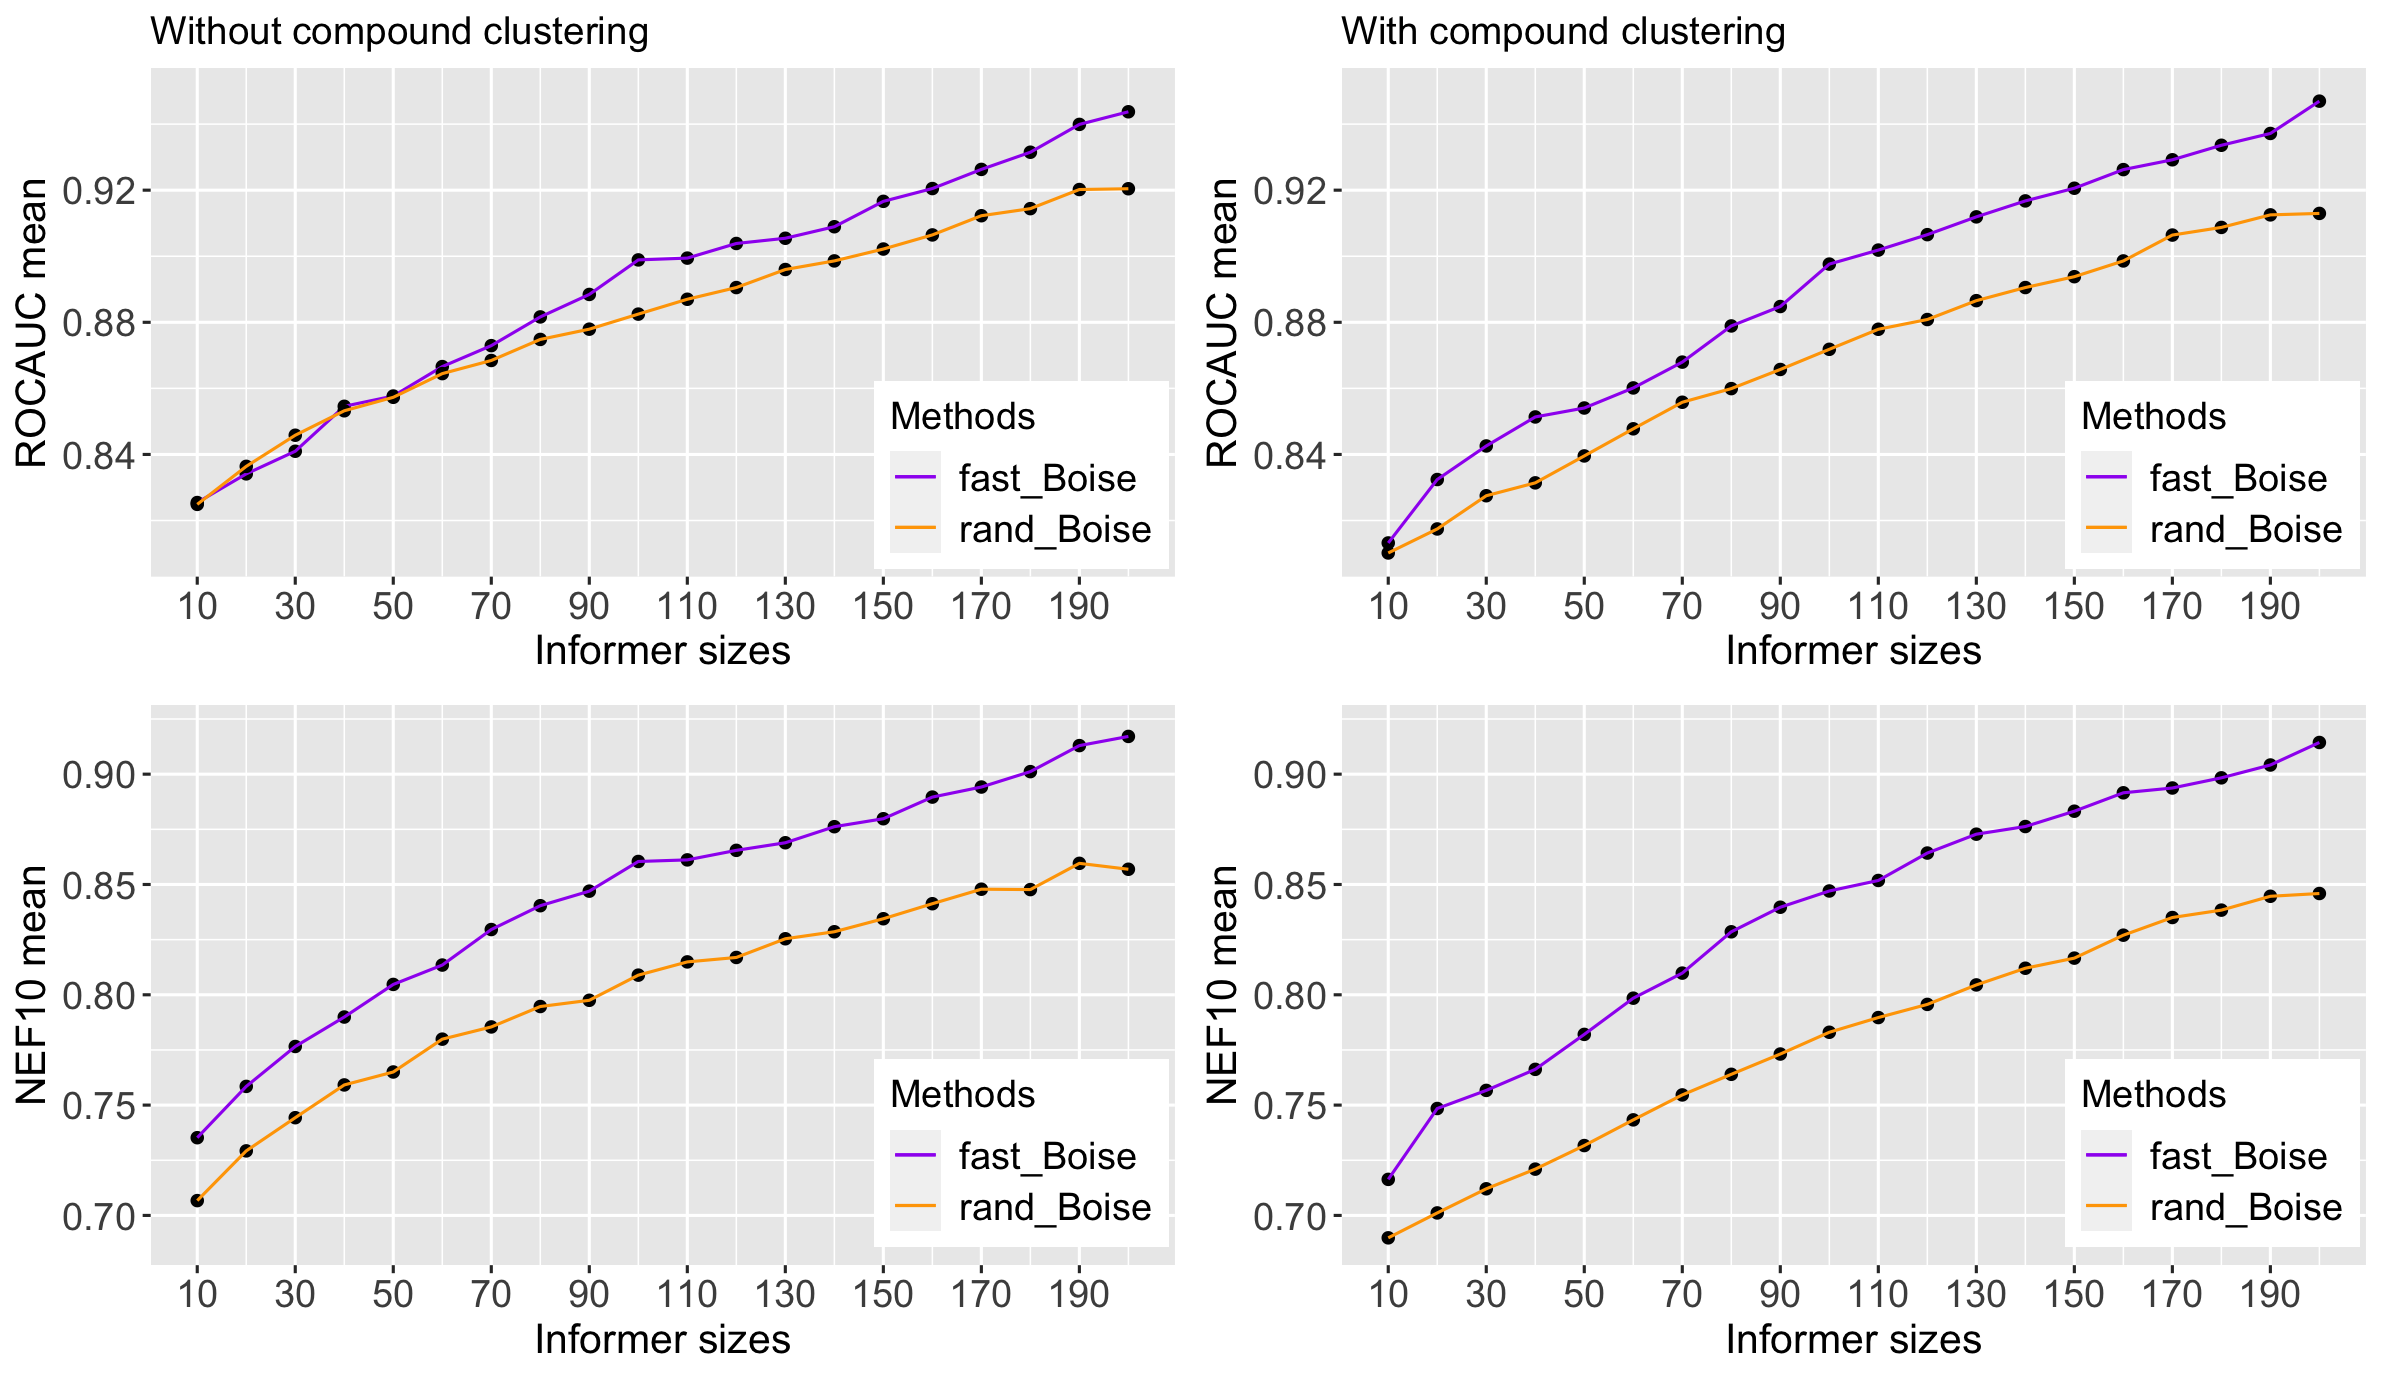
\includegraphics[width=5.0in]{Figs/fast_entropy_pel1_rand_200_informers.png}
\caption{\label{fig:fast_rand_200_informer} 
{\bf Comparison of fast BOISE and randomly selected informers with and without compound clustering $\mathcal G$ when $n_A$ ranging from $10$ to $200$}.}
\end{figure}



\subsubsection{Prospective analysis}
Following the retrospective analysis on FDA data set, we further test the BOISE variants on a few more targets in a prospective way. A prospective analysis can help prevent the look-ahead bias and give us an estimate of BOISE variants performances in a real-world scenario. There are $6$ chemical screening labs who test FDA approved drugs on their interested targets, and they kindly made $18$ novel targets available to us. A brief summary of these novel targets is in Table~\ref{tab:lab_tgt_summary}. 

\begin{table}[ht!]
\centering
\caption{\label{tab:lab_tgt_summary}
{\bf Summary of $18$ novel targets in prospective analysis}}
\begin{tabular}{  p{3cm}  p{2cm}  p{3cm} p{6cm}}
        \toprule
\textbf{Lab name}  
& \textbf{Target IDs}
& \textbf{Target types}
& \textbf{Protocol description}\\\midrule
Ahlquist
& 1 to 4
& Cell
& Yeast growth inhibition assay, OD600 measurement;
\\\hline

Hoskins
& 5
& Cell
& AFUMSF3B1 with FDA library, OD600 measurement;
\\\hline

Hull
& 6 to 10
& Spores and fungal cell
& 10h and 22h Germination with FDA plates; 12h yeast with FDA plates;
\\\hline

Keck
& 11 to 16
& AlphaScreen assay, FP assay and cell
& Selleck FDA library screen using AlphaScreen assay of Biotin-SSB-Ct peptide interaction and fluorescence polarization assay of FAM-SSB-Ct peptide interaction with 6x-His Klebsiella pneumoniae DnaG (KpnDnaG) primase and PriA (KpnPriA) helicase;
\\\hline

Senes
& 17
& Protein
& Raw alpha screen
\\\hline

Xing
& 18
& Protein
& MTDH-SND1 for FDA screen; His-CFP-SND1(16-336), 0.8 uM His-YFP-MTDH(386-407), 12.8 uM compound, 60uM
\\\hline
\bottomrule
\end{tabular}
\end{table}

The prospective test on these $18$ targets follows exactly the same procedures as in Figure~\ref{fig:IBR_scheme}: at the very beginning, nothing is known about the targets except for which FDA compounds will be tested against them. Various informer sets are then selected for each target using different BOISE variants, with informer sizes the same as in retrospective analysis. We provide these informer sets to collaborators and they give us the actual bioactivity responses on each target. After that, rankings of all tested FDA compounds are given based on initial $x_0$ and intermediate $x_A$ and we evaluate these rankings on the true outcomes. 

The performances of BOISE variants in prospective analysis are similar to those in retrospective analysis: the mean and median of NEF10 and ROCAUC are almost the same for original BOISE with $L_1(\cdot)$ loss. Block BOISE performs better prospectively than retrospectively, and original BOISE with $L_2(\cdot)$ loss is slightly worse, probably due to its sensitivity to violation of model assumptions. Block BOISE achieves best average performance on both NEF10 and ROCAUC in this prospective analysis. All three variants mentioned above are better than fast BOISE, although the difference is not significant. After having the full bioactivity data on novel targets, we also test the baseline rand-BOISE where $30$ informers are randomly sampled, and it is still worse than all the BOISE variants. Table~\ref{tab:recovery_counts} below shows the number of hits recovered within top $100$ ranked compounds under different methods for each of $18$ novel targets, and Figure~\ref{fig:prospective_compar} is a summary of ROCAUC and NEF10 in this prospective analysis.

\bigskip
\begin{table}[ht!]
\centering
\caption{\label{tab:recovery_counts}
{\bf Number of hits recovered by different BOISE variants in their top 100 ranked compounds on $18$ novel targets using FDA data set.} The novel targets are sorted based on their total number of hits in FDA compounds. The recovery counts of rand-BOISE is the average of $25$ randomly selected informer sets.}

\begin{tabular}{ ccccccc }
\multicolumn{1}{c}{ID} & \multicolumn{1}{c}{rand-BOISE} & \multicolumn{1}{c}{fast BOISE} & \multicolumn{1}{c}{orig BOISE(L2)} & \multicolumn{1}{c}{block BOISE} & 
\multicolumn{1}{c}{orig BOISE(L1)} & 
\multicolumn{1}{c}{total} \\
 \hline
 18 & 4.60 & 4 & 4 & 5 & 4 & 6 \\
 15 & 6.04 & 6 & 6 & 6 & 6 & 7 \\
 14 & 6.96 & 7 & 7 & 7 & 7 & 8 \\
 11 & 5.76 & 7 & 7 & 6 & 7 & 9 \\
 3 & 5.76 & 6 & 7 & 8 & 7 & 14 \\
 12 & 8.04 & 10 & 6 & 8 & 11 & 15 \\
 17 & 8.00 & 10 & 10 & 9 & 10 & 16 \\
 4 & 8.08 & 8 & 12 & 12 & 12 & 17 \\
 16 & 9.92 & 11 & 9 & 12 & 11 & 18 \\
 13 & 7.80 & 7 & 9 & 12 & 10 & 20 \\
 5 & 11.84 & 8 & 13 & 17 & 12 & 23 \\
 1 & 12.52 & 17 & 15 & 16 & 18 & 27 \\
 6 & 11.80 & 13 & 13 & 17 & 9 & 28 \\
 2 & 16.40 & 23 & 19 & 21 & 21 & 35 \\
 10 & 16.12 & 18 & 21 & 21 & 20 & 36 \\
 9 & 13.92 & 17 & 16 & 20 & 16 & 38 \\
 7 & 12.28 & 14 & 14 & 17 & 16 & 48 \\
 8 & 16.28 & 14 & 19 & 22 & 19 & 53 \\
\end{tabular}\\
\end{table}
\bigskip

\begin{figure}[!ht]
\centering
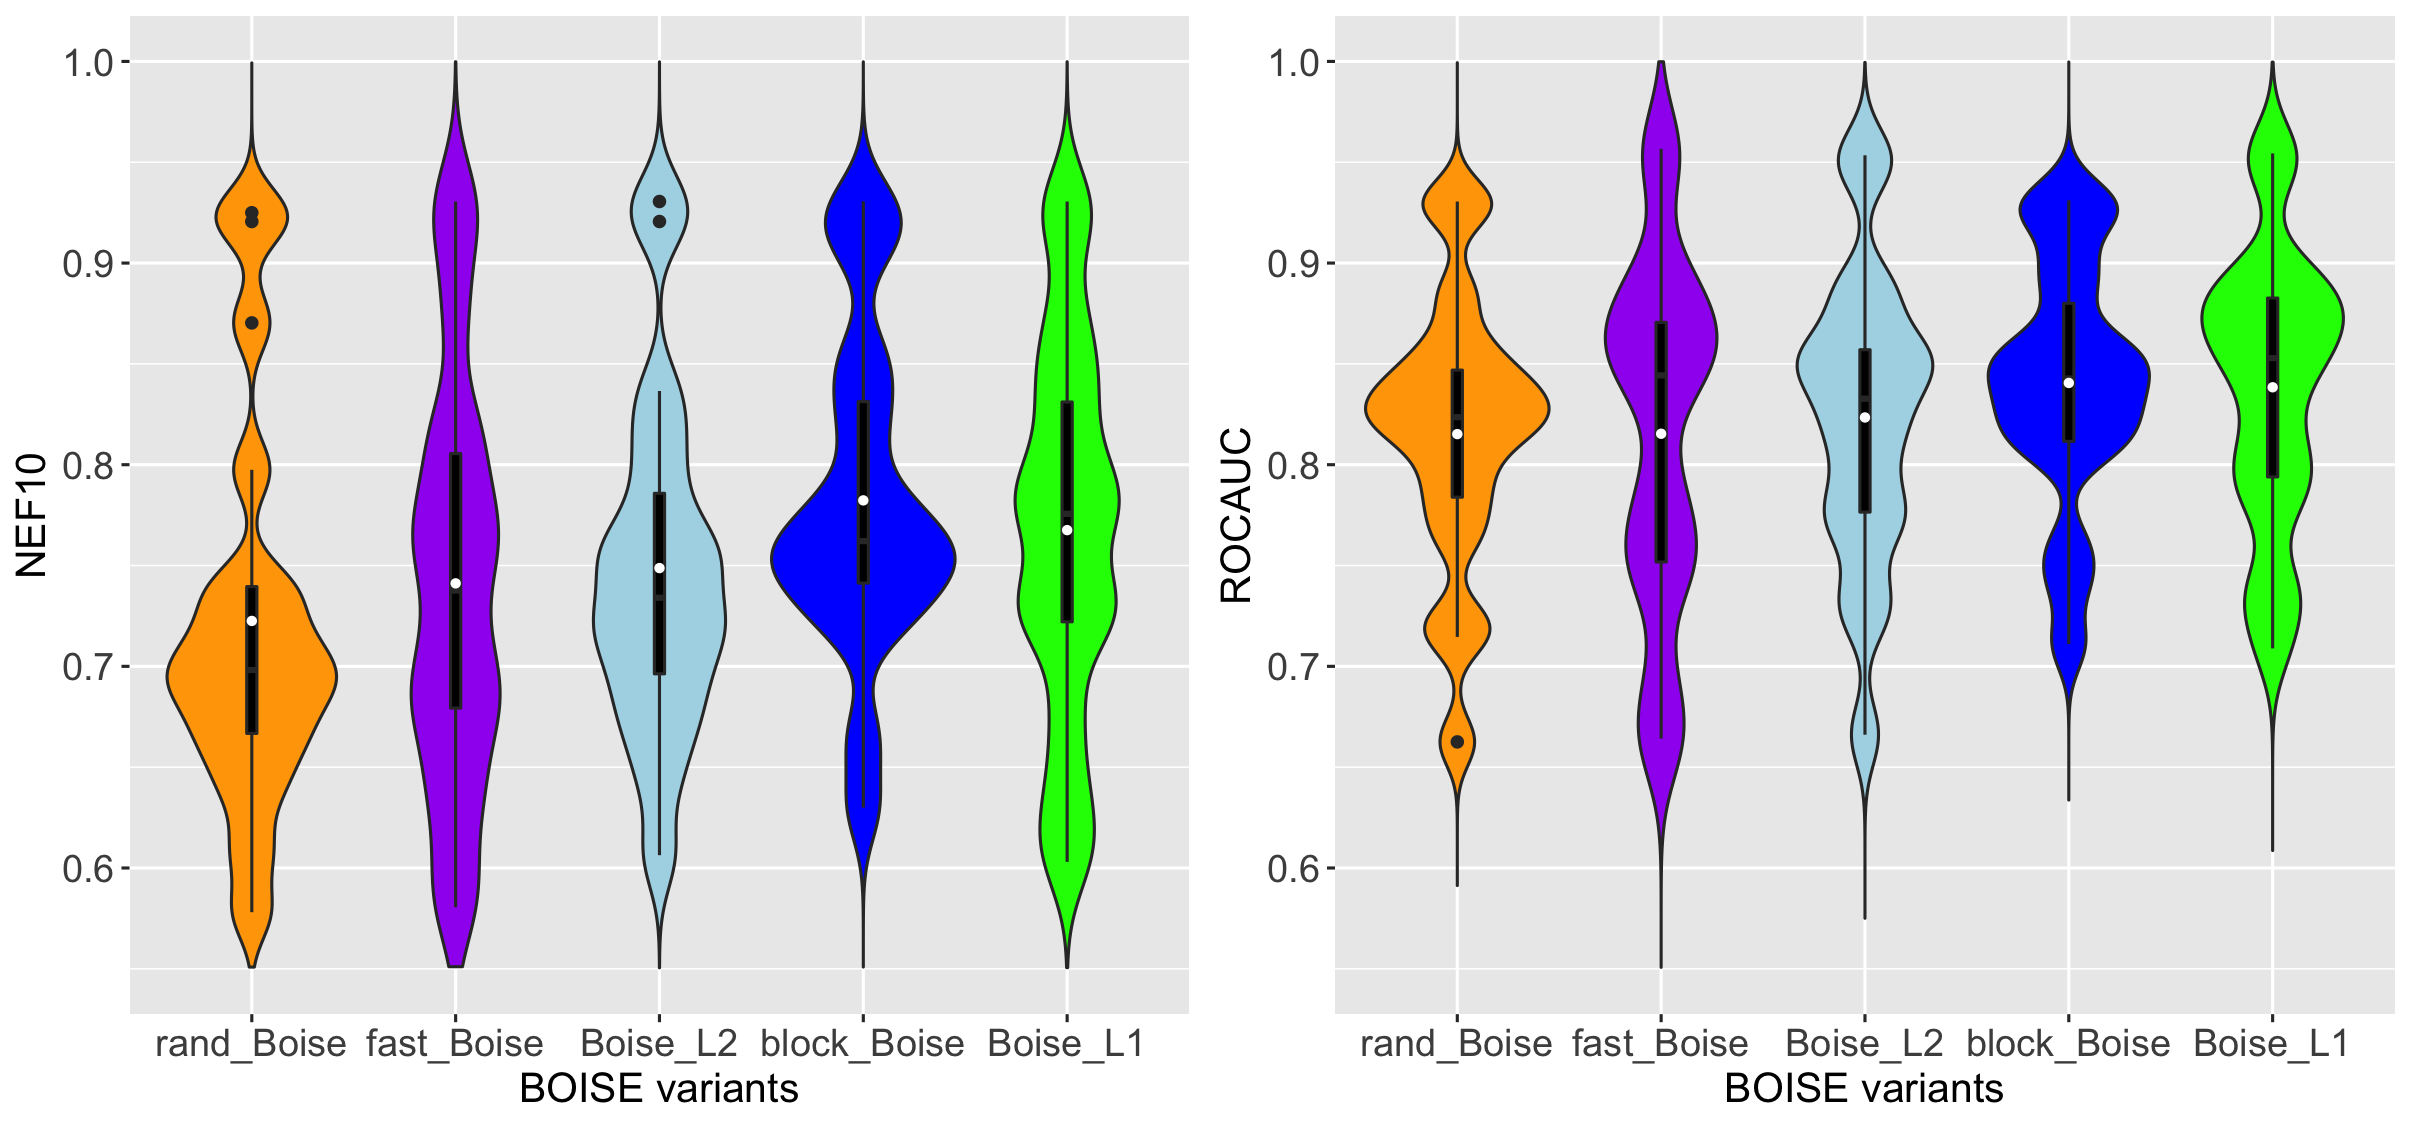
\includegraphics[width=5.0in]{Figs/prospective_nef_roc_compar.png}
\caption{\label{fig:prospective_compar} 
{\bf Summary of performances of BOISE variants in prospective analysis.} All methods are applied on $18$ novel targets, with FDA data set as initial bioactivity data $x_0$. The informer set sizes are the same as in retrospective analysis, with $n_A=20$ for original BOISE methods and $n_A = 30$ for block BOISE, fast BOISE and baseline rand-BOISE.}
\end{figure}

\subsection{PCBA data set}
The PCBA data set is a bioacitivity data matrix used in real drug discovery research, which is first introduced by \cite{pcba_Ramsundar_2015} from PubChem library. In this experiment, a condensed version of PCBA is used with most missing values removed due to the limitation of computer memory. The condensed PCBA data contains $102$ targets and $134264$ compounds, with a missing rate of $5.4\%$ and active rate of $0.7\%$. We apply fast BOISE method on this PCBA data to further test its scalability and compare it with naive informers that are frequently used by biochemistry researchers. The experiment is conducted in the same retrospective and prospective way as on FDA data set, with $30$ targets randomly selected from PCBA data set as test targets, and one novel target used to test fast BOISE prospectively. The results on fast BOISE, as aforementioned, provide the guidance of how other BOISE variants perform and how many informers are enough for PCBA.

Previous experiments on FDA data show that fast BOISE performs slightly better without compound clustering $\mathcal G$, thus a target grouping on the whole bioactivity matrix is in favor. However, floating point error due to large number of compounds makes sampling algorithm of CRP extremely inefficient. On that account, we approximate the posterior sampling of CRP by randomizing the distance matrix as suggested in the appendix of \cite{Ma_approximate_CRP_2021}. The distance matrix is defined by Jaccard distance on complete responses between two targets, and the number of clusters for a randomized distance matrix is selected by validity score with threshold of $0.9$, following the same procedure in the original paper. With this approximate sampling of CRP, we compare fast BOISE with randomly selected informers for $n_A = 100,200,500$ and $1000$ on 30 test targets. The ROCAUC and NEF1 results are illustrated with scatterplots in Fig~\ref{fig:pcba_fast_random_roc} and Fig~\ref{fig:pcba_fast_random_nef}, respectively, and the majority of points ($\approx 22/30$) are above the diagonal line, assuring the superiority of fast BOISE over random selections.
\begin{figure}[!ht]
\centering
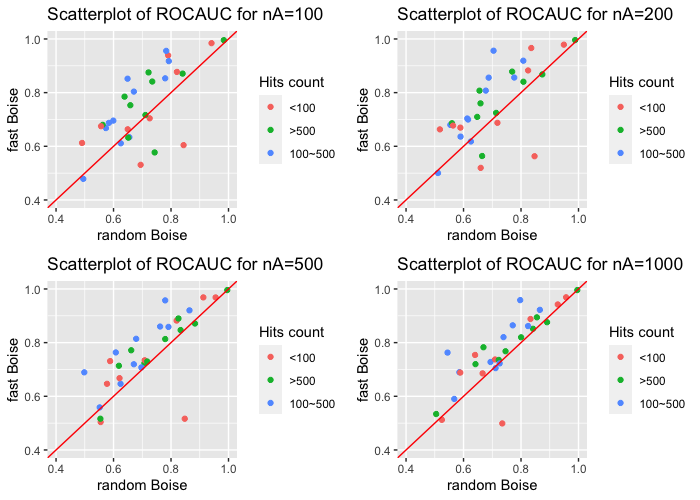
\includegraphics[width=5.0in]{Figs/random_entropy_roc_compar.png}
\caption{\label{fig:pcba_fast_random_roc} 
{\bf ROCAUC comparison of fast BOISE and randomly selected informers on $30$ test targets from PCBA data set for $n_A = 100, 200, 500$ and $1000$. }}
\end{figure}

\begin{figure}[!ht]
\centering
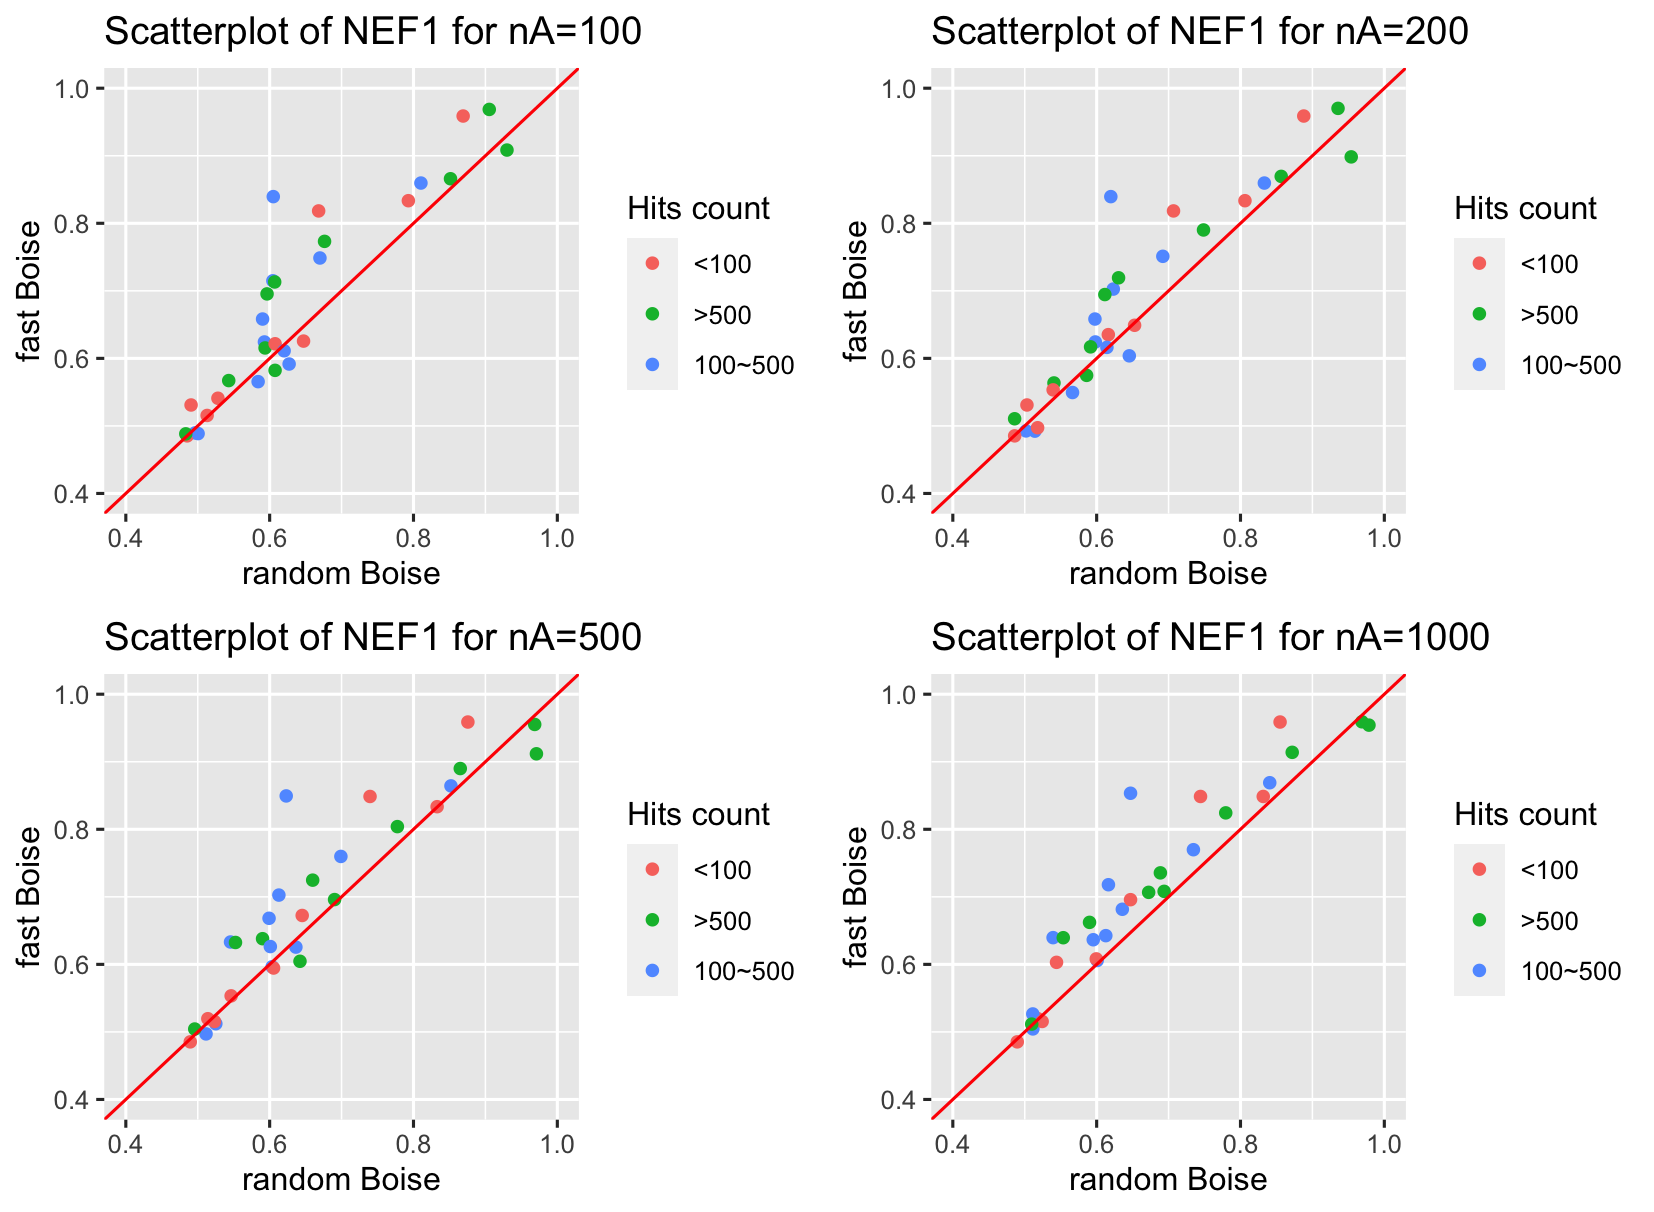
\includegraphics[width=5.0in]{Figs/random_entropy_nef1_compar.png}
\caption{\label{fig:pcba_fast_random_nef} 
{\bf NEF1 comparison of fast BOISE and randomly selected informers on $30$ test targets from PCBA data set for $n_A = 100, 200, 500$ and $1000$. }}
\end{figure}

In practice, biochemistry researchers often use FDA approved drugs as the starting point when assessing a novel target. These drugs serve a similar role as the informer set in IBR. In condensed PCBA data set, $324$ compounds overlap with the FDA data. Fig~\ref{fig:pcba_fast_fda} is the comparison between fast BOISE and these FDA approved informers on $30$ test targets, with informer size of fast BOISE kept the same as the number of available FDA approved compounds for each target. Among $30$ test targets, fast BOISE achieves a better ROCAUC on $26$, a better NEF1 on $23$, and the same NEF1 on $3$ targets, implying a potential boost in ranking accuracy if the role of FDA approved drugs is replaced with informers selected by BOISE methods. 

\begin{figure}[!ht]
\centering
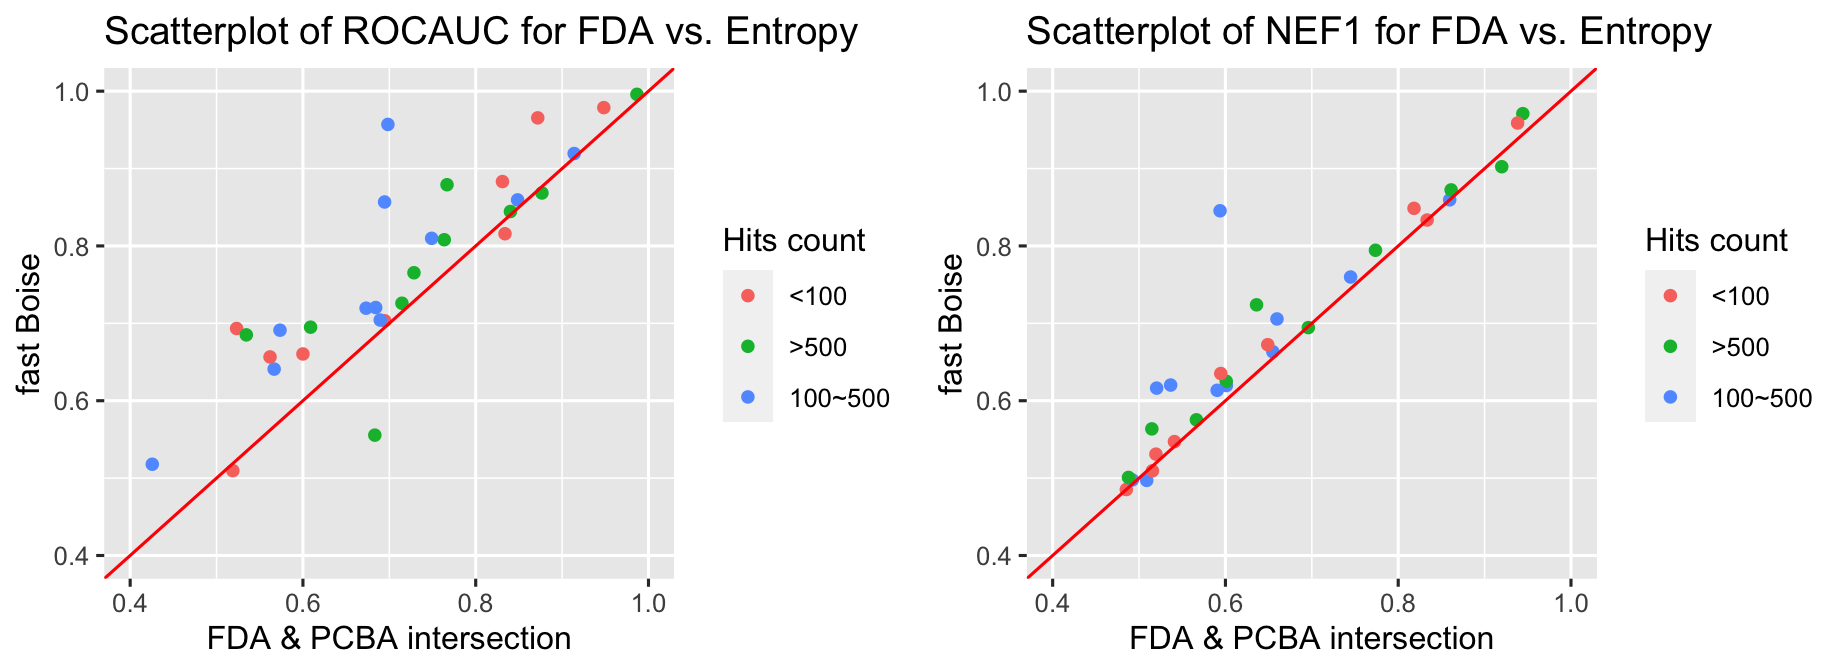
\includegraphics[width=5.0in]{Figs/fda_entropy_compar.png}
\caption{\label{fig:pcba_fast_fda} 
{\bf Comparison of fast BOISE and informers using FDA approved drugs on $30$ test targets from PCBA data set.} The informer size of fast BOISE is the same as the number of FDA approved compounds with non-missing values on each test target.}
\end{figure}

When evaluated prospectively, a novel target, PriA-SSB, is tested on most of the compounds in PCBA and is predicted by fast BOISE method. 
PriA-SSB is a bacteria protein-protein interaction target that has been tested on $114081$ out of $134264$ PCBA compounds~\citep{alnammi_evaluating_2021}. As for FDA approved drugs, there are $253$ drugs that are tested on both PriA-SSB and the other $102$ targets in PCBA data set. 
In this prospective analysis, an approximate CRP sampling is similarly applied on the whole PCBA data set for fast BOISE method, which is later compared with naive informer sets like randomly selected informers and FDA-approved informers on PriA-SSB. 
The NEF1 and ROCAUC results are summarized in following Table~\ref{tab:pcba_prospective}. The result is not so impressive as in retrospective analysis, where fast BOISE is better than FDA approved drugs on both NEF1 and ROCAUC, and achieves a better NEF1 but slightly worse ROCAUC than randomly selected informers.

\begin{table}[htbp]
\caption{\label{tab:pcba_prospective}  {\bf Prospective comparison between fast BOISE and naive informer set on novel target PriA-SSB}. The informer size $n_A = 253$ is for informer set that consists of FDA-approved drugs, and $n_A = 500, 1000$ is for randomly selected informer sets.}
\begin{tabular}{r|rrr}
\multicolumn{1}{c}{informer size $n_A$} & 
\multicolumn{1}{c}{253} & 
\multicolumn{1}{c}{500} & 
\multicolumn{1}{c}{1000} 
\\
 \hline
 NEF1-fast &  $0.553$ & $0.605$ & $0.622$ \\
 NEF1-random &  $0.564$ & $0.542$ & $0.533$ \\
 NEF1-FDA &  $0.536$ & -- & -- \\
 ROCAUC-fast & $0.862$ & $0.883$ & $0.890$ \\
 ROCAUC-random & $0.890$ & $0.891$ & $0.893$ \\
 ROCAUC-FDA & $0.838$ & -- & -- \\
 \hline
\end{tabular}
\end{table}

A further investigation explains the mediocre performance of fast BOISE on PriA-SSB.
After clustering the $102$ targets from PCBA through CRP, a $103\times 103$ matrix could be used to illustrate the frequency at which each pair of targets are grouped together,
where the last target (the 103rd column) is a ``fake" target that represents the unknown new cluster that potentially exists but no one belongs to. 
The left panel in Figure~\ref{fig:pcba_prospective_clustering} shows this ``adjacency frequency" from our approximate CRP clustering after rearrangement, where darker color indicates that pair of targets are more frequently grouped together. 
There are a few blocks in the plot, meaning that some targets are highly correlated and hence always clustered together in CRP. 

After selecting informers through fast BOISE and getting the intermediate data $x_A$ on PriA-SSB, we can compute the posterior probability on which each of $103$ targets will be potentially grouped with PriA-SSB. The posterior probabilities act like the similarity between each target and the novel target. 
The right panel in Figure~\ref{fig:pcba_prospective_clustering} plots a weighted adjacency frequency of $103$ targets, where weights are those posterior probabilities. 
This plot aims to find groups of targets (i.e. dark blocks) that are most similar to the novel target based on CRP clustering, and the conclusion is astonishing: it says PriA-SSB is most similar to Target ID 103, the ``fake" target representing targets outside PCBA.
Therefore, fast BOISE claims that PriA-SSB is not similar to any existing target clusters in PCBA and we should not use PCBA data set to predict results on PriA-SSB. That explains why the performance is not so impressive as in retrospective analysis. 

\begin{figure}[!ht]
\centering
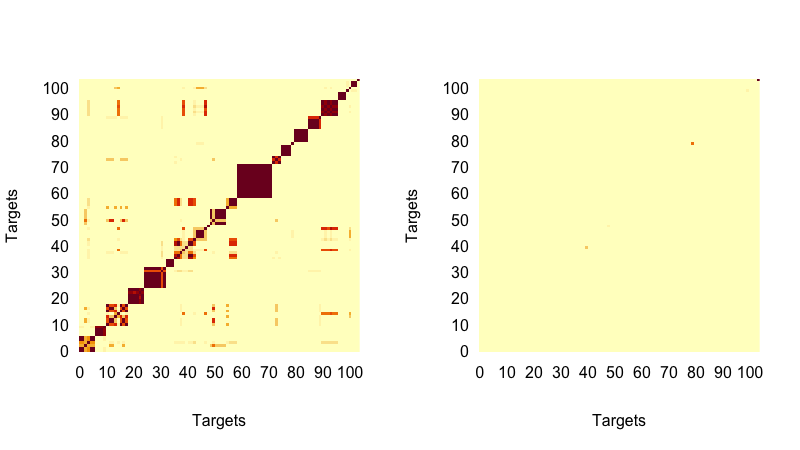
\includegraphics[width=5.0in]{Figs/Adj_matices.png}
\caption{\label{fig:pcba_prospective_clustering} 
{\bf Adjacency frequencies with approximate CRP clustering on PCBA (left), and a weighted version of the same clustering with weights representing similarity to PriA-SSB (right).} The left plot shows the adjacency frequency from the approximate CRP clustering after rearrangement, where darker color indicates that pair of targets are more frequently grouped together and blocks indicate groups of targets that are highly correlated. The right plot shows a weighted adjacency frequency of the same clustering, where weights are posterior probabilities of each target being grouped with PriA-SSB. The last ``target" (the 103rd column) is a fake target that represents the unknown new cluster that potentially exists but no one belongs to. }
\end{figure}


For a novel target not in existing target clusters, if we are forced to give a prediction with current data, the best we can do is to give a simple prediction with the aggregated data, and it turns out the simplest ranking method is the best on PriA-SSB.
For example, if we forget about CRP or informer selection and simply rank all the compounds with their average active rates in PCBA data set, this ranking achieves $0.657$ on NEF1 and $0.955$ on ROCAUC for PriA-SSB, both better than any method in Table~\ref{tab:pcba_prospective}. 

\section{Discussion}
BOISE is an effective IBR method that characterize the virtual screening procedure as a statistical decision problem. The advantage of BOISE comes from a combination of Bayes decision theory and flexible statistical model. 
Despite being the most effective IBR method, a limitation of BOISE is the computation complexity, which impedes its application to real-world large scale virtual screening. Scalability is crucial in virtual screening, especially in early stage drug discovery where millions of compounds are to be screened. There is a trade-off between accuracy and scalability, however, the fact that BOISE performs better than heuristic IBR methods suggests potential improvement over na\'ive informer selection when scaling up BOISE. 

The proposed BOISE variants, block BOISE and fast BOISE, solve the scaling problem to various degrees: 
block BOISE aims for enormous chemical space but small informer set, while fast BOISE is recommended for larger informer sets. 
The idea of block BOISE is to generalize traditional BOISE, where initial bioactivity data is broken into separate blocks. A  degenerate case of block BOISE is exactly the original BOISE. Therefore, block BOISE achieves a balance between computation cost and prediction accuracy. For example, it is the best method on ROCAUC in both retrospective and prospective analysis, while only costing $1/6$ as much time as needed for original BOISE method. 
Fast BOISE, on the other hand, origins from the analysis of informers selected. It is related to original BOISE but operates on a totally different family of loss functions. 
The most significant improvement of fast BOISE is its non-sequential selection of informers, which can save a lot of time when the informer set size is large. It is not a good idea to use non-sequential selection in regard to prediction accuracy, as correlation among informers is not taken into account. 
However, fast BOISE achieves comparable predictive performances in both retrospective and prospective analyses, indicating that it could serve as a lower bound of the performance for BOISE-like methods and a reference for experimental designs. 

There are also a few gaps found between theory and practice for original BOISE. Being the Bayes rule only guarantees the optimal decision rule under given loss function, and that doesn't necessarily lead to a decent IBR method, as shown for frequent-hitters rule in Section~2.1.4. The proposed new loss function $L_1(A, T; x_{i^*})$ resolves the issue where inactive compounds tested in intermediate data can still be ranked top in the final ranking. The improvement is consistent in both synthetic data and case studies, and persists even when model assumptions are violated to different degrees. We then upgrade original BOISE with $L_1(A, T; x_{i^*})$ throughout the case studies. Another proposed loss function, $L_2(A, R; x_{i^*})$, utilizes a pairwise ranking loss for justification of the ranking procedure. BOISE with $L_2(A, R; x_{i^*})$ loss is expected to have best overall ranking performance in theory, and it is true when model assumptions are mostly satisfied. However, the performance is quite sensitive to the structure of initial bioactivity data $x_0$, as is shown in synthetic data. The sensitivity is also proved in FDA case study, where it is the best method on ROCAUC retrospectively, but merely above fast BOISE prospectively. For the reason of potential violations of target-clustering model~(\ref{eq:orig_model_structure}), loss function $L_1(A, T; x_{i^*})$ may be preferred over $L_2(A, R; x_{i^*})$. 

In prospective analysis on FDA data, an apparent performance discrepancy appears among target types, although the computation does not include such information. 
In average, most BOISE variants perform better on molecule-level targets like AlphaScreen / FP assays and protein targets; the performance degrades on cell-level targets like spores and fungal cells. 
It is less related to chemical screening labs: for example, targets 11 to 16 are all from Keck's lab, and target 13 is a cell target while the others are molecule-level targets. Although other targets are always among the best performed targets throughout the prospective analysis, performance on target 13 is usually just around the average and inferior to performances on protein targets from other labs. 
The discrepancy among target types indicates that there is a more direct relationship between compound structure and bioactivity for molecule-level assays. For cellular assays, where the readout is often OD600, chemical screening researchers are basically just looking at how well visible light passes through the medium, where liquid gets more clear on cell death. For cell death, there might be many molecular mechanisms that produce a positive readout. 
A careful selection of targets may be helpful in constructing the initial bioactivity matrix $x_0$, as it may be confusing to mix molecular targets and cellular targets in a single bioactivity matrix.

\clearpage
\bibliographystyle{biom}	
%{\footnotesize
\bibliography{bibliography}        
%} 
\end{document}
